\documentclass[conference]{IEEEtran}

% ---------- Packages ----------
\usepackage[T1]{fontenc}
\usepackage[utf8]{inputenc}
\usepackage{cite}
\usepackage{graphicx}
\usepackage{amsmath,amssymb}
\usepackage{booktabs}
\usepackage{array}
\usepackage{xcolor}
\usepackage{url}
\usepackage{float}
\usepackage{caption}
\usepackage{subcaption}
\usepackage{enumitem}
\usepackage{hyperref}

\hypersetup{
    colorlinks=true,
    linkcolor=blue,
    citecolor=blue,
    urlcolor=blue
}

% ---------- Custom Notes ----------
\newcommand{\gemininote}[1]{\textcolor{purple}{\textbf{Note (Gemini Deep Research Output):} #1}}

% ---------- Custom visible marker for editable section ----------
\newcommand{\ideaheader}[1]{
    \vspace{0.5em}
    \noindent
    \colorbox{black}{\parbox{\dimexpr\columnwidth-2\fboxsep\relax}{\centering\color{white}\textbf{#1}}}
    \vspace{0.5em}
}

\begin{document}

\title{Visualizing Uncertainty in GPS and Location Data\\
for Uncertainty-Aware Decision Support}

\author{
\IEEEauthorblockN{Mustafa Bozyel}
\IEEEauthorblockN{Senih Kırmaç }
\IEEEauthorblockN{Ömer Mert Özel}
\IEEEauthorblockA{
Computer Science and Engineering\\
Sabancı University\\
Istanbul, Turkey\\
mustafa.bozyel@sabanciuniv.edu
}
}

\maketitle

\begin{abstract}
This mock proposal focuses on the visualization of uncertainty in GPS and location-based data within the broader context of uncertainty-aware decision support. Rather than reducing uncertainty, the goal is to represent it explicitly in a way that is understandable and useful for users. The report introduces the problem context, reviews related studies on uncertainty visualization with an emphasis on geospatial and positional ambiguity, and prepares the ground for possible visualization approaches that will later be proposed and evaluated.
\end{abstract}

\begin{IEEEkeywords}
uncertainty visualization, GPS uncertainty, location data, geospatial visualization, decision support, human-centered computing
\end{IEEEkeywords}

\section{Introduction}

The broader graduation project topic is \textit{AI-Driven Uncertainty-Aware Visualization for Decision Making Under Stress}. Within this scope, our specific interest is the visualization of uncertainty in GPS and location data.

In many real-world systems, location information is displayed as if it were exact, even when the underlying data is noisy, incomplete, inferred, or semantically ambiguous. This may create false confidence and lead users to over-trust the output. Therefore, our aim is not primarily to reduce uncertainty, but to \textbf{make uncertainty visible}.

A motivating example is a case where a bank transaction appears to come from a shopping mall such as Akasya AVM, while the true location may correspond to one of many stores inside that area. Similarly, a GPS reading may point to a single coordinate even though the actual position could lie somewhere within a larger uncertain region.

The main research question of this proposal is the following:

\begin{quote}
How can uncertainty in GPS and location-based data be visualized in a way that is honest, interpretable, and useful for decision-making?
\end{quote}

\section{Problem Scope and Initial Interpretation}

Based on the first meeting notes, the main direction of the project is uncertainty representation rather than uncertainty elimination. The initial discussion suggests three relevant directions:

\begin{enumerate}[leftmargin=1.5em]
    \item \textbf{GPS uncertainty:} how to display uncertainty in positional data,
    \item \textbf{Density-related ambiguity:} uncertainty in regions with high concentration of data, although this direction is currently not the main focus,
    \item \textbf{Model-generated uncertainty:} uncertainty arising from Gaussian or other probabilistic models used to generate or infer location distributions.
\end{enumerate}

Among these, the most central and manageable direction for now is GPS and positional uncertainty. Thus, the first step is to examine prior work on how researchers visualize ambiguous, probabilistic, or approximate spatial data.

\section{Background: Why Location Data is Uncertain}

GPS and location data may be uncertain for many reasons, including sensor noise, signal loss, multipath effects in dense urban areas, temporal delay, map-matching errors, coarse aggregation, and model-based inference.

For this project, uncertainty can be interpreted under several categories:

\begin{itemize}[leftmargin=1.5em]
    \item \textbf{Positional uncertainty:} the real position may lie within an area rather than at a single point,
    \item \textbf{Semantic uncertainty:} a general place is known but the exact sub-location is unknown,
    \item \textbf{Model uncertainty:} the algorithm producing the estimate has uncertainty of its own,
    \item \textbf{Temporal uncertainty:} the recorded position may not exactly match the time of the event.
\end{itemize}

These categories will help us compare related work and later define suitable visualization strategies.

\section{Publication Search and Related Work}

This section summarizes the publications that are most directly related to our problem of visualizing uncertainty in GPS and location-based data. We focus especially on work involving degraded GPS, positional ambiguity, self-location judgments, and concrete visual encodings that can later inspire our own design alternatives.

\subsection{Visualising Location Uncertainty to Support Navigation under Degraded GPS Signals: a Comparison Study}

Ranasinghe et al.\ proposed two new visualizations for location uncertainty in pedestrian navigation and compared them with existing methods in a field-based user study. Their results showed that the new visualizations reduced wrong turns, and users especially preferred the landmark-based design for judging their true location under degraded GPS conditions \cite{ranasinghe2019visualising}.

This paper is highly useful for our project because it directly studies how uncertainty in mobile location data can be communicated during navigation. It is particularly relevant since it evaluates visual designs not only conceptually, but also in terms of user performance and acceptance, which can help us justify our own visualization choices.

\begin{figure}[t]
    \centering
    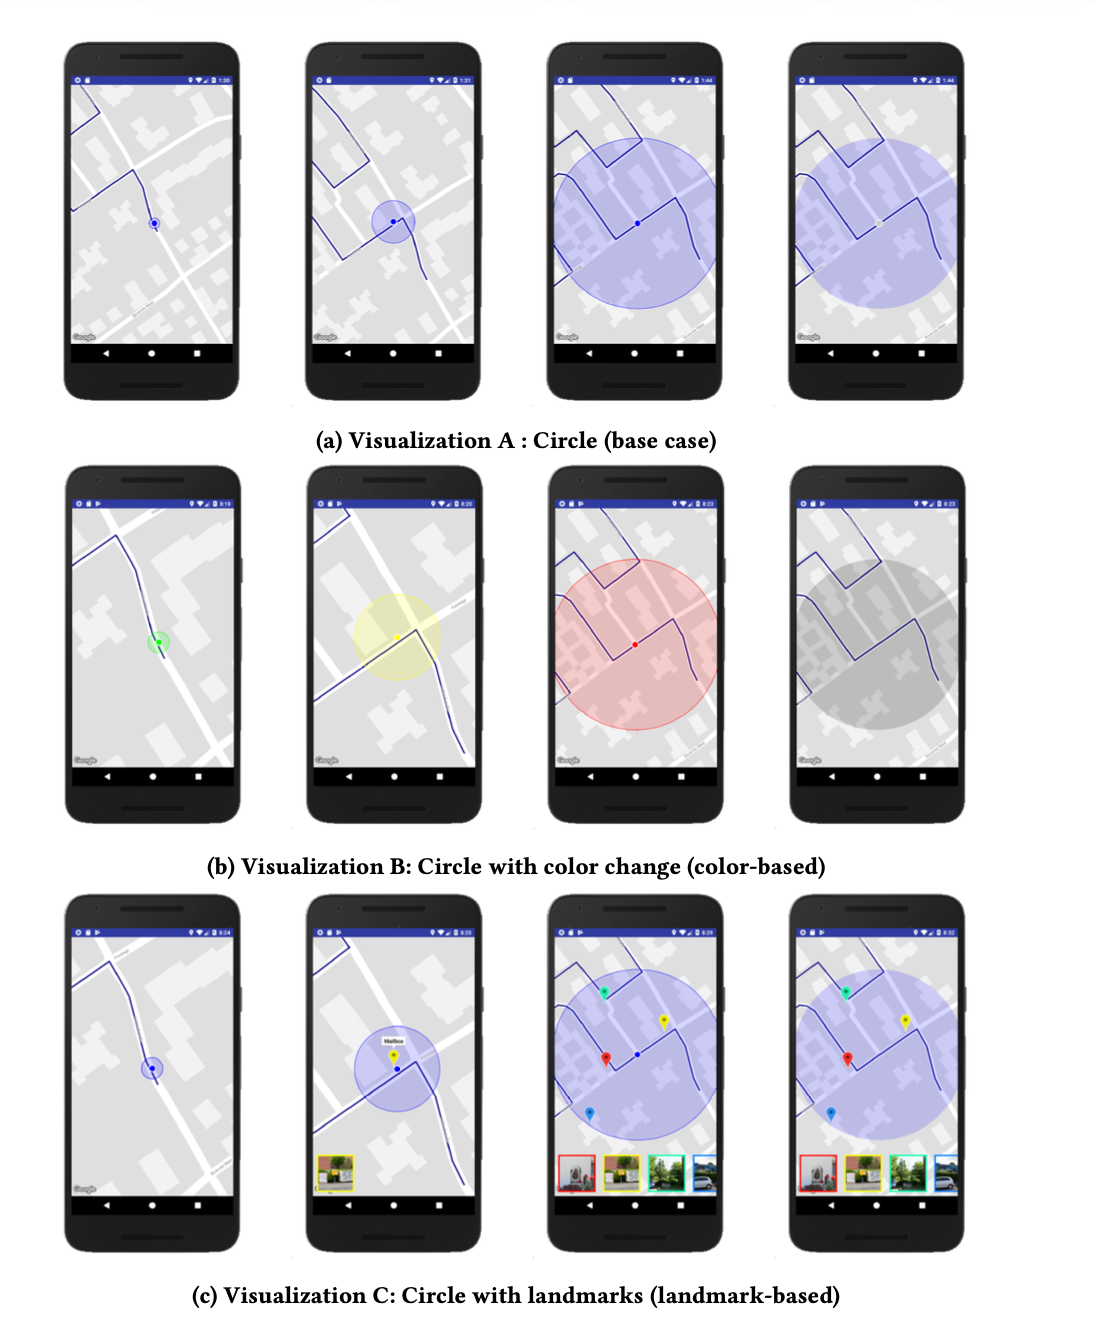
\includegraphics[width=\linewidth]{images/fig_ranasinghe2019_visualizations.png}
    \caption{Location uncertainty visualizations compared by Ranasinghe et al.\ for pedestrian navigation under degraded GPS signals \cite{ranasinghe2019visualising}.}
    \label{fig:ranasinghe2019}
\end{figure}

\subsection{Pedestrian Navigation with Degraded GPS Signal: Investigating the Effects of Visualizing Position Uncertainty}

Burigat and Chittaro investigated whether uncertainty visualizations help users navigate when GPS signals are inaccurate or unavailable. They compared a basic display with two dynamic uncertainty visualizations, namely a circular uncertainty region and colored street segments, and found that the street-coloring approach reduced workload and was perceived as more beneficial \cite{burigat2011pedestrian}.

This source is highly relevant because it addresses almost the same design problem as ours: how to present uncertain user position in a map-based interface. It is especially useful for thinking about whether uncertainty should be shown as an area around the user or projected onto meaningful map structures such as roads or regions.

\begin{figure}[t]
    \centering
    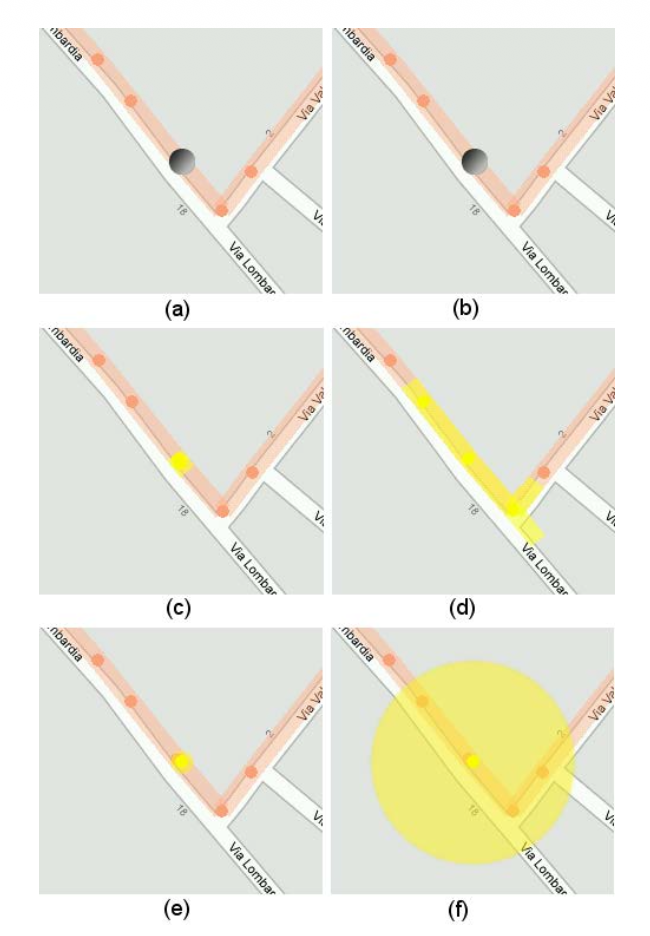
\includegraphics[width=\linewidth]{images/fig_burigat2011_navigation_uncertainty.png}
    \caption{Alternative uncertainty displays for pedestrian navigation, including circular and street-based encodings \cite{burigat2011pedestrian}.}
    \label{fig:burigat2011}
\end{figure}

\subsection{Assessing the Effectiveness of Different Visualizations for Judgments of Positional Uncertainty}

McKenzie et al.\ examined four alternative visualizations for positional uncertainty in a mobile mapping scenario inspired by Google’s blue dot. They compared uniform blue circles and Gaussian fades, each with or without a visible centroid dot, and found that the uniform blue circle led to judgments that were both faster and more consistent with the underlying probability distribution \cite{mckenzie2016assessing}.

This paper is very useful for our work because it directly compares glyph-based encodings for uncertain self-location. It can help us decide whether simple shapes, faded probability-style visuals, or centroid markers are better for communicating uncertainty in a map interface.

\begin{figure}[t]
    \centering
    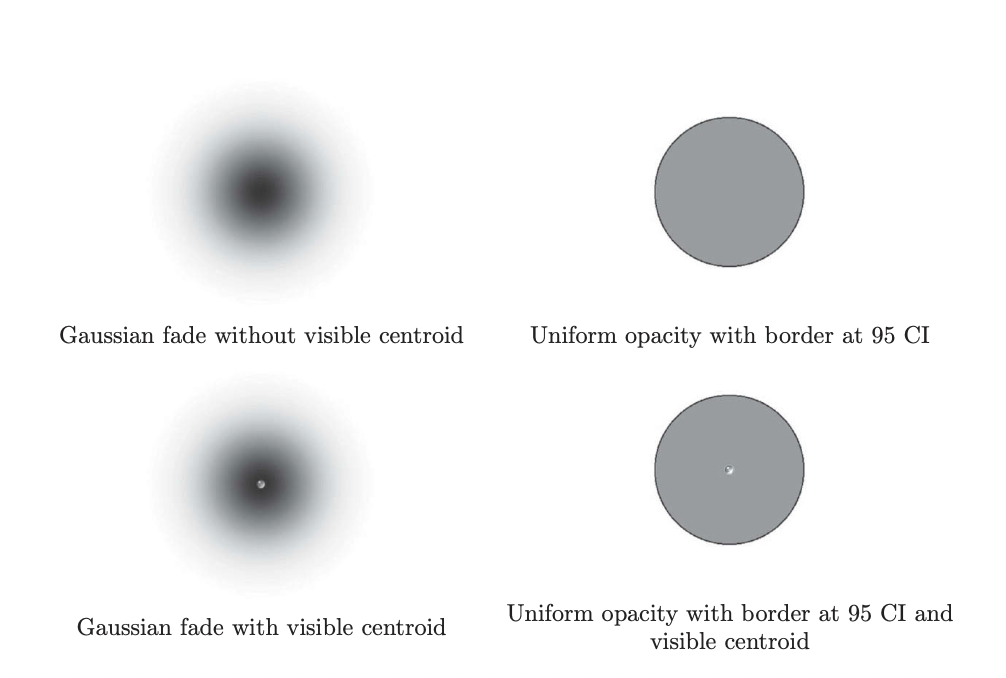
\includegraphics[width=\linewidth]{images/fig_mckenzie2016_blue_dot_variants.png}
    \caption{Alternative blue-dot style visualizations for positional uncertainty judgments \cite{mckenzie2016assessing}.}
    \label{fig:mckenzie2016}
\end{figure}

\subsection{Where Are You? The Effect of Uncertainty and Its Visual Representation on Location Judgments in GPS-Like Displays}

Hegarty et al.\ studied how nonexpert users interpret positional uncertainty on GPS-like displays. They compared circle-based confidence displays and faded glyphs representing probability density, and found that users generally assumed the center as the most likely location while combining multiple uncertain estimates in intuitive but task-dependent ways \cite{hegarty2016where}.

This source is relevant because our project also concerns how people reason about uncertain location data rather than only how uncertainty is computed mathematically. The paper is particularly valuable for understanding user strategies and for showing that the best visual encoding may depend on the decision task.

\begin{figure}[t]
    \centering
    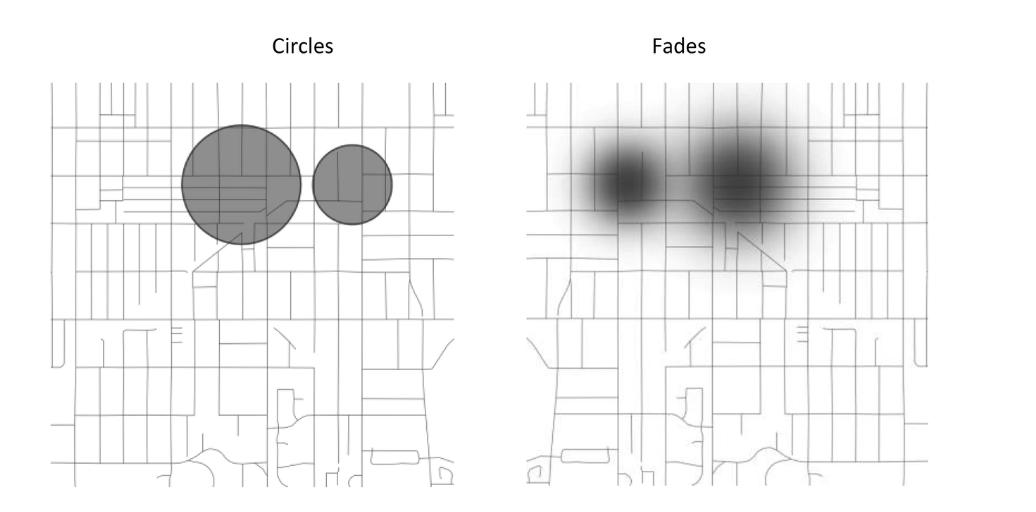
\includegraphics[width=\linewidth]{images/fig_hegarty2016_location_judgment_displays.png}
    \caption{GPS-like uncertainty representations used for location judgment tasks \cite{hegarty2016where}.}
    \label{fig:hegarty2016}
\end{figure}

\subsection{Visualization of Spatio-Temporal GPS Uncertainty within a GIS Environment}

Lodha et al.\ focused on measuring, modeling, and visualizing the uncertainty of GPS-tracked objects registered within a GIS environment. They modeled horizontal position, speed, and direction errors, and visualized the uncertainty of moving objects using diffused object representations over aerial imagery \cite{lodha2002visualization}.

This paper is useful for our project because it provides an early but highly relevant GPS-specific example of uncertainty visualization in a geospatial environment. It is especially valuable for thinking about spatio-temporal uncertainty and for understanding how uncertain trajectories or tracked objects might be represented beyond a single point estimate.

\begin{figure}[t]
    \centering
    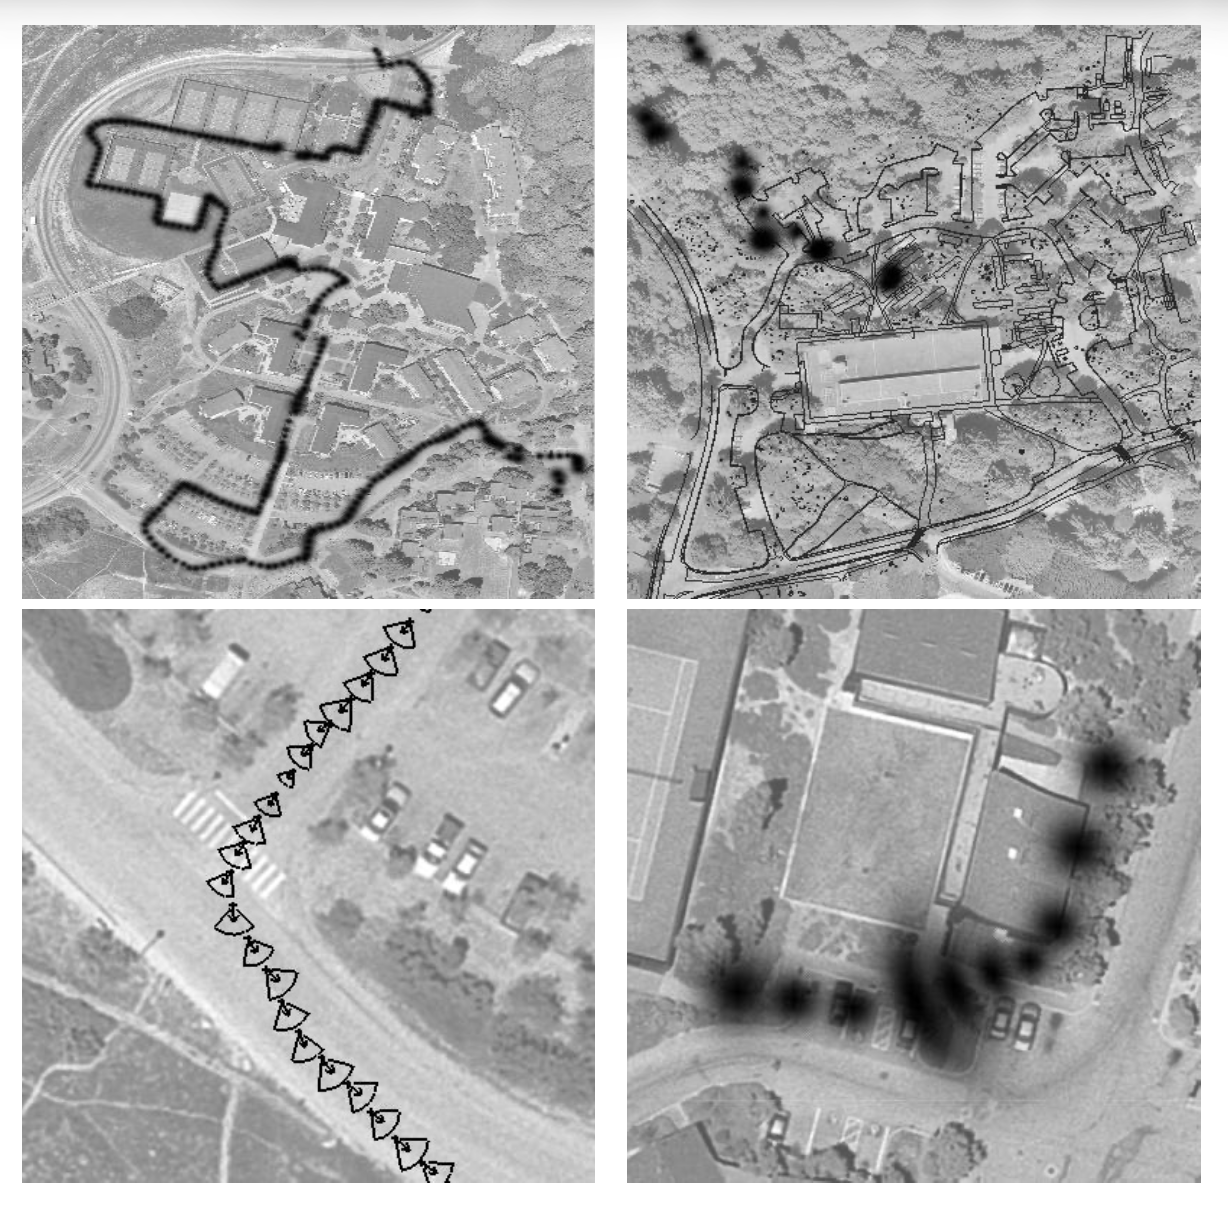
\includegraphics[width=\linewidth]{images/fig_lodha2002_gps_uncertainty_gis.png}
    \caption{Example of spatio-temporal GPS uncertainty visualization within a GIS environment \cite{lodha2002visualization}.}
    \label{fig:lodha2002}
\end{figure}


\section{Possible Visualization Directions}

Based on the initial project framing and the reviewed literature, several possible approaches may later be explored for representing uncertainty in GPS and location data:

\begin{itemize}[leftmargin=1.5em]
    \item confidence circles or ellipses around uncertain points,
    \item blurred or semi-transparent markers,
    \item probability heatmaps or probability surfaces,
    \item multiple candidate positions,
    \item region-based highlighting for semantically ambiguous locations,
    \item animation-based encodings for uncertainty strength,
    \item interval or range-based location representations.
\end{itemize}

These ideas will be refined after the literature review is expanded.

\section{Planned Methodology}

The project will proceed in several stages.

\subsection{Literature Review}
We will review publications on uncertainty visualization, with priority given to geospatial data, cartography, GPS error visualization, and probabilistic interfaces.

\subsection{Design Space Exploration}
We will identify and compare visual encoding methods that may effectively communicate uncertainty in location data.

\subsection{Candidate Solution Development}
We will later define possible visualization solutions for our own system based on the reviewed literature and project requirements.

\subsection{Evaluation Criteria}
The candidate approaches may be compared in terms of interpretability, clarity, honesty of uncertainty communication, scalability, and cognitive load.

\section{Our Visualization Ideas}

This section presents our own visualization concepts for improving how uncertainty is shown in GPS and map-based interfaces. The traditional blue-dot metaphor usually represents uncertainty as a uniformly blurred circular area. While this gives a rough sense of positional ambiguity, it does not explain whether some parts of the uncertainty region are more likely than others. Our ideas aim to make this internal structure of uncertainty more visible and more informative for users.

Our first idea is a \textbf{probability-weighted boundary representation}. In this design, the uncertainty region is still shown as a circular area, but the boundary is not visually uniform. Instead, the edge becomes thicker or bolder only in the portions of the circle that correspond to more probable location areas. This allows the visualization to preserve the familiar circular uncertainty metaphor while adding an extra layer of meaning. Rather than treating the whole perimeter equally, the interface highlights the boundary segments associated with higher likelihood.

Our second idea is an \textbf{internal density-based uncertainty representation}. In this concept, the uncertainty circle is enriched by emphasizing more likely subregions inside the circle with stronger contrast or denser shading. In other words, the uncertain area is not visualized as a single homogeneous zone. Instead, it contains internal regions with different levels of likelihood. This representation is not limited to directional emphasis only; it can also communicate that some irregular or local areas within the uncertainty region are more plausible than others.

Together, these two ideas explore two complementary ways of improving uncertainty visualization. The first focuses on the \emph{boundary} of the uncertainty region by strengthening the edges of more probable areas, while the second focuses on the \emph{interior structure} by showing varying likelihood within the region itself. Both approaches attempt to move beyond the standard uniform blue-dot model and provide users with a richer understanding of possible location estimates.

\begin{figure}[t]
    \centering
    \begin{subfigure}{\columnwidth}
        \centering
        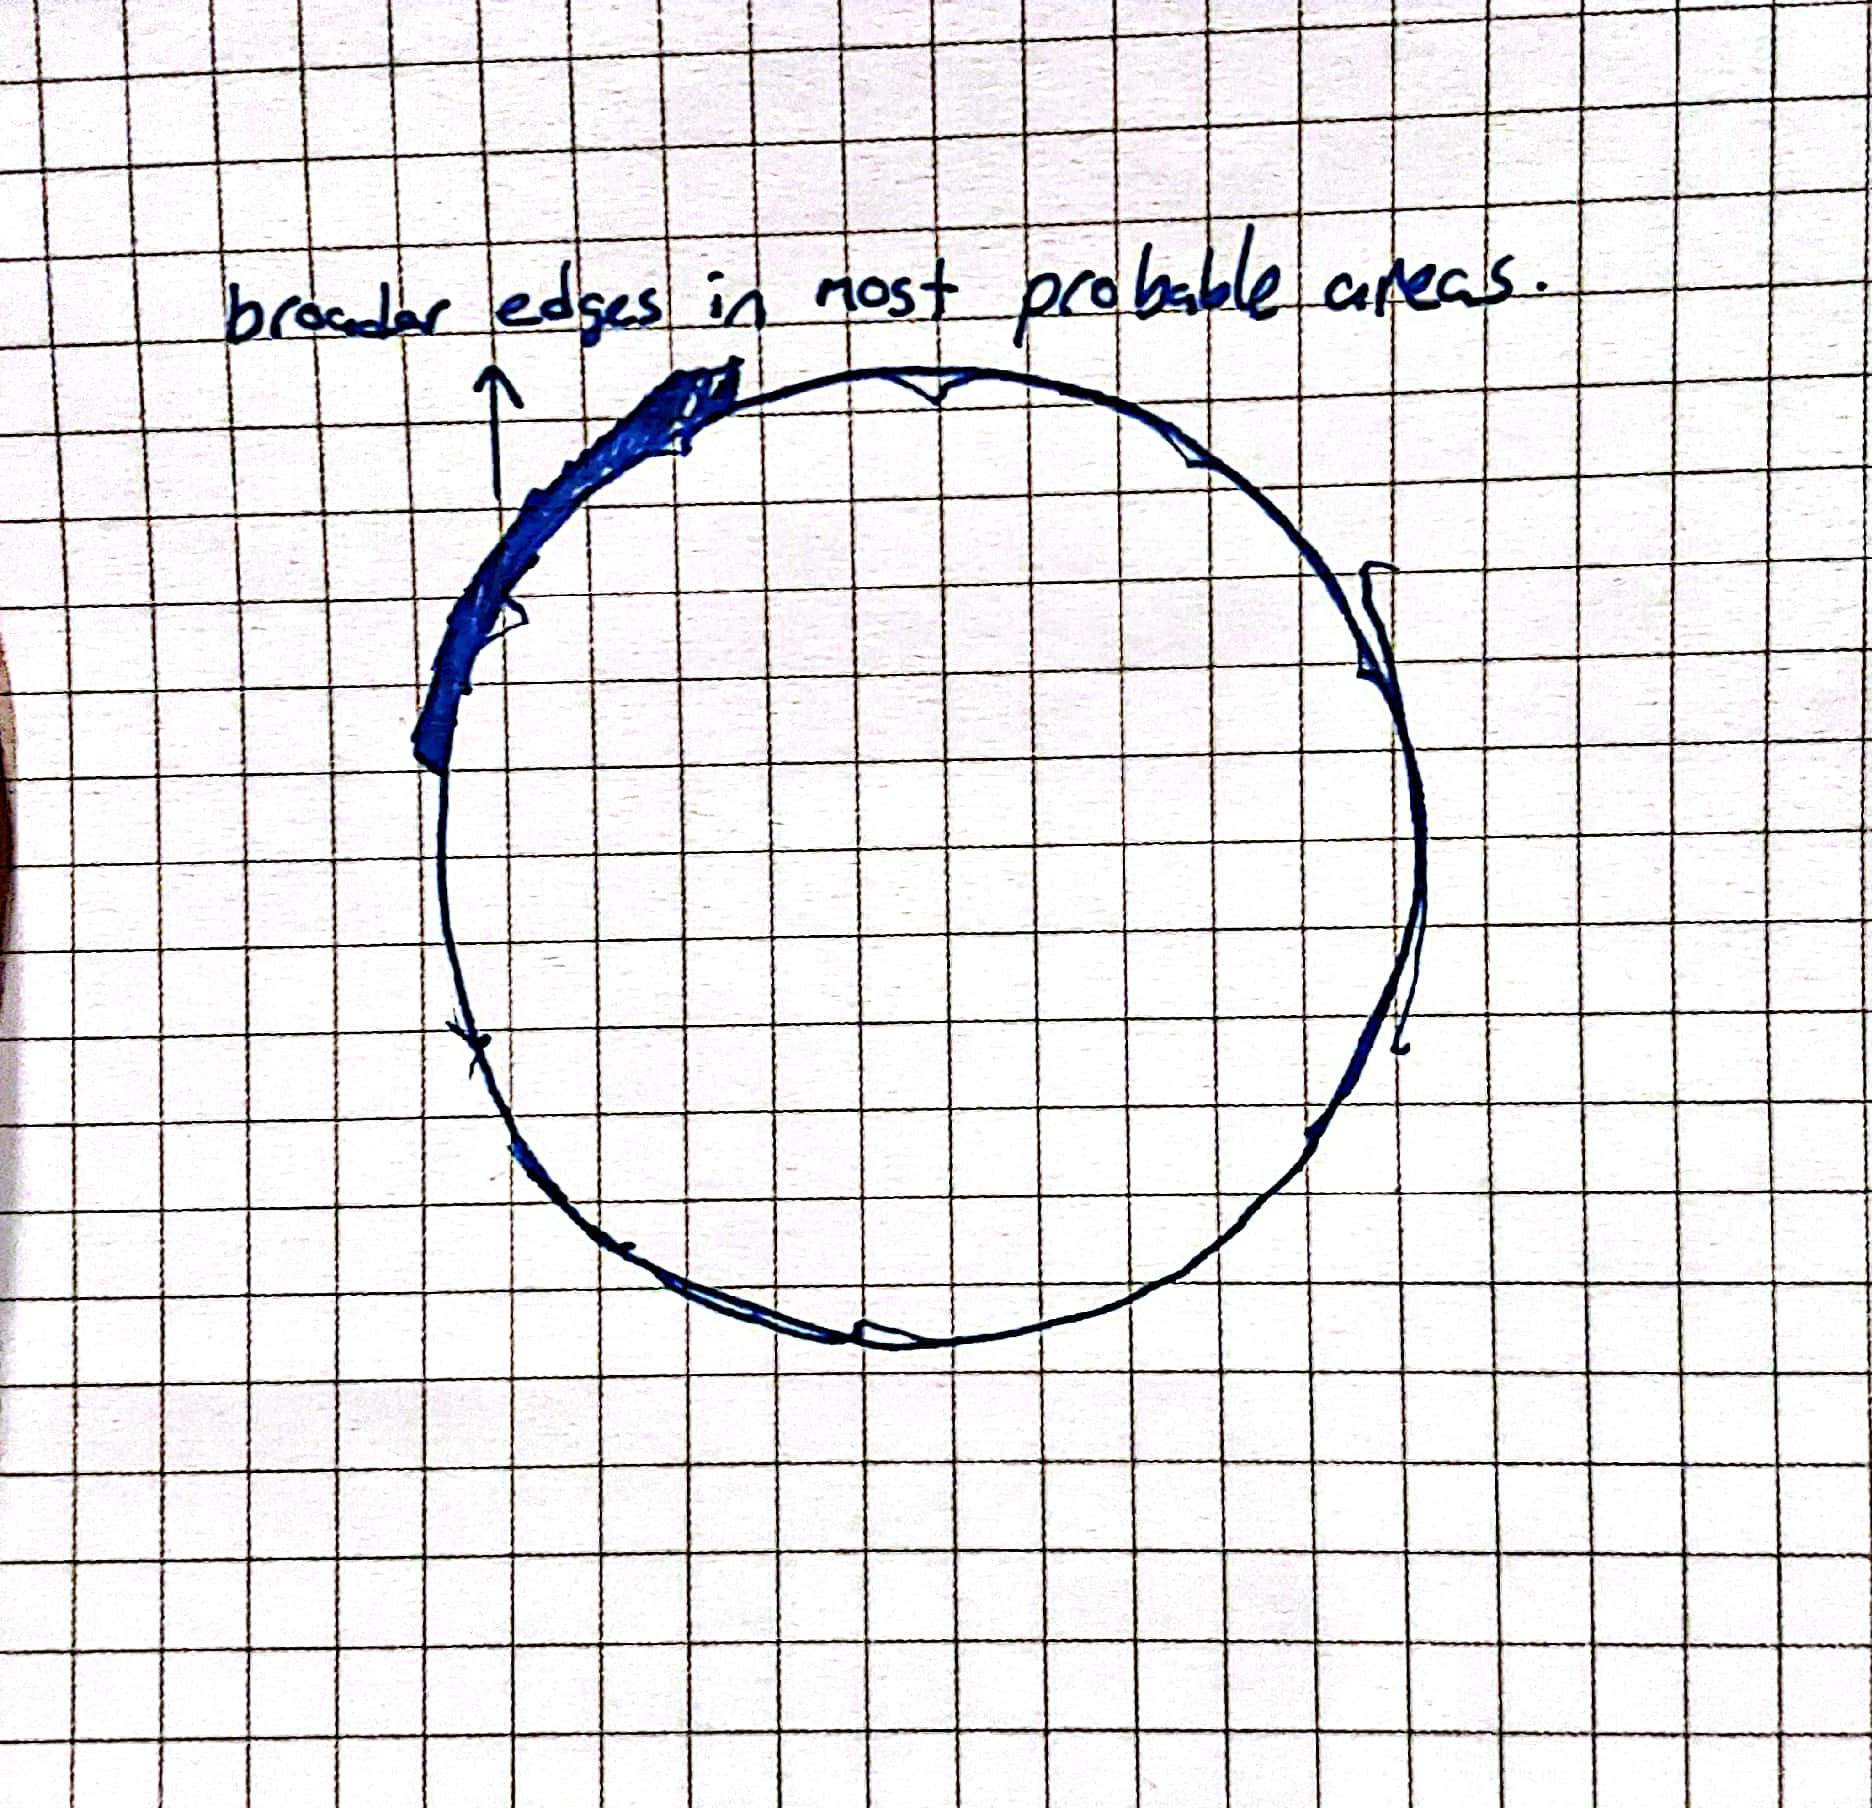
\includegraphics[width=0.95\columnwidth]{images/directional-edge.jpeg}
        \caption{Probability-weighted boundary concept. The circular uncertainty region is preserved, but the edge is thicker in the parts corresponding to more probable areas.}
        \label{fig:directional_edge}
    \end{subfigure}

    \vspace{0.5em}

    \begin{subfigure}{\columnwidth}
        \centering
        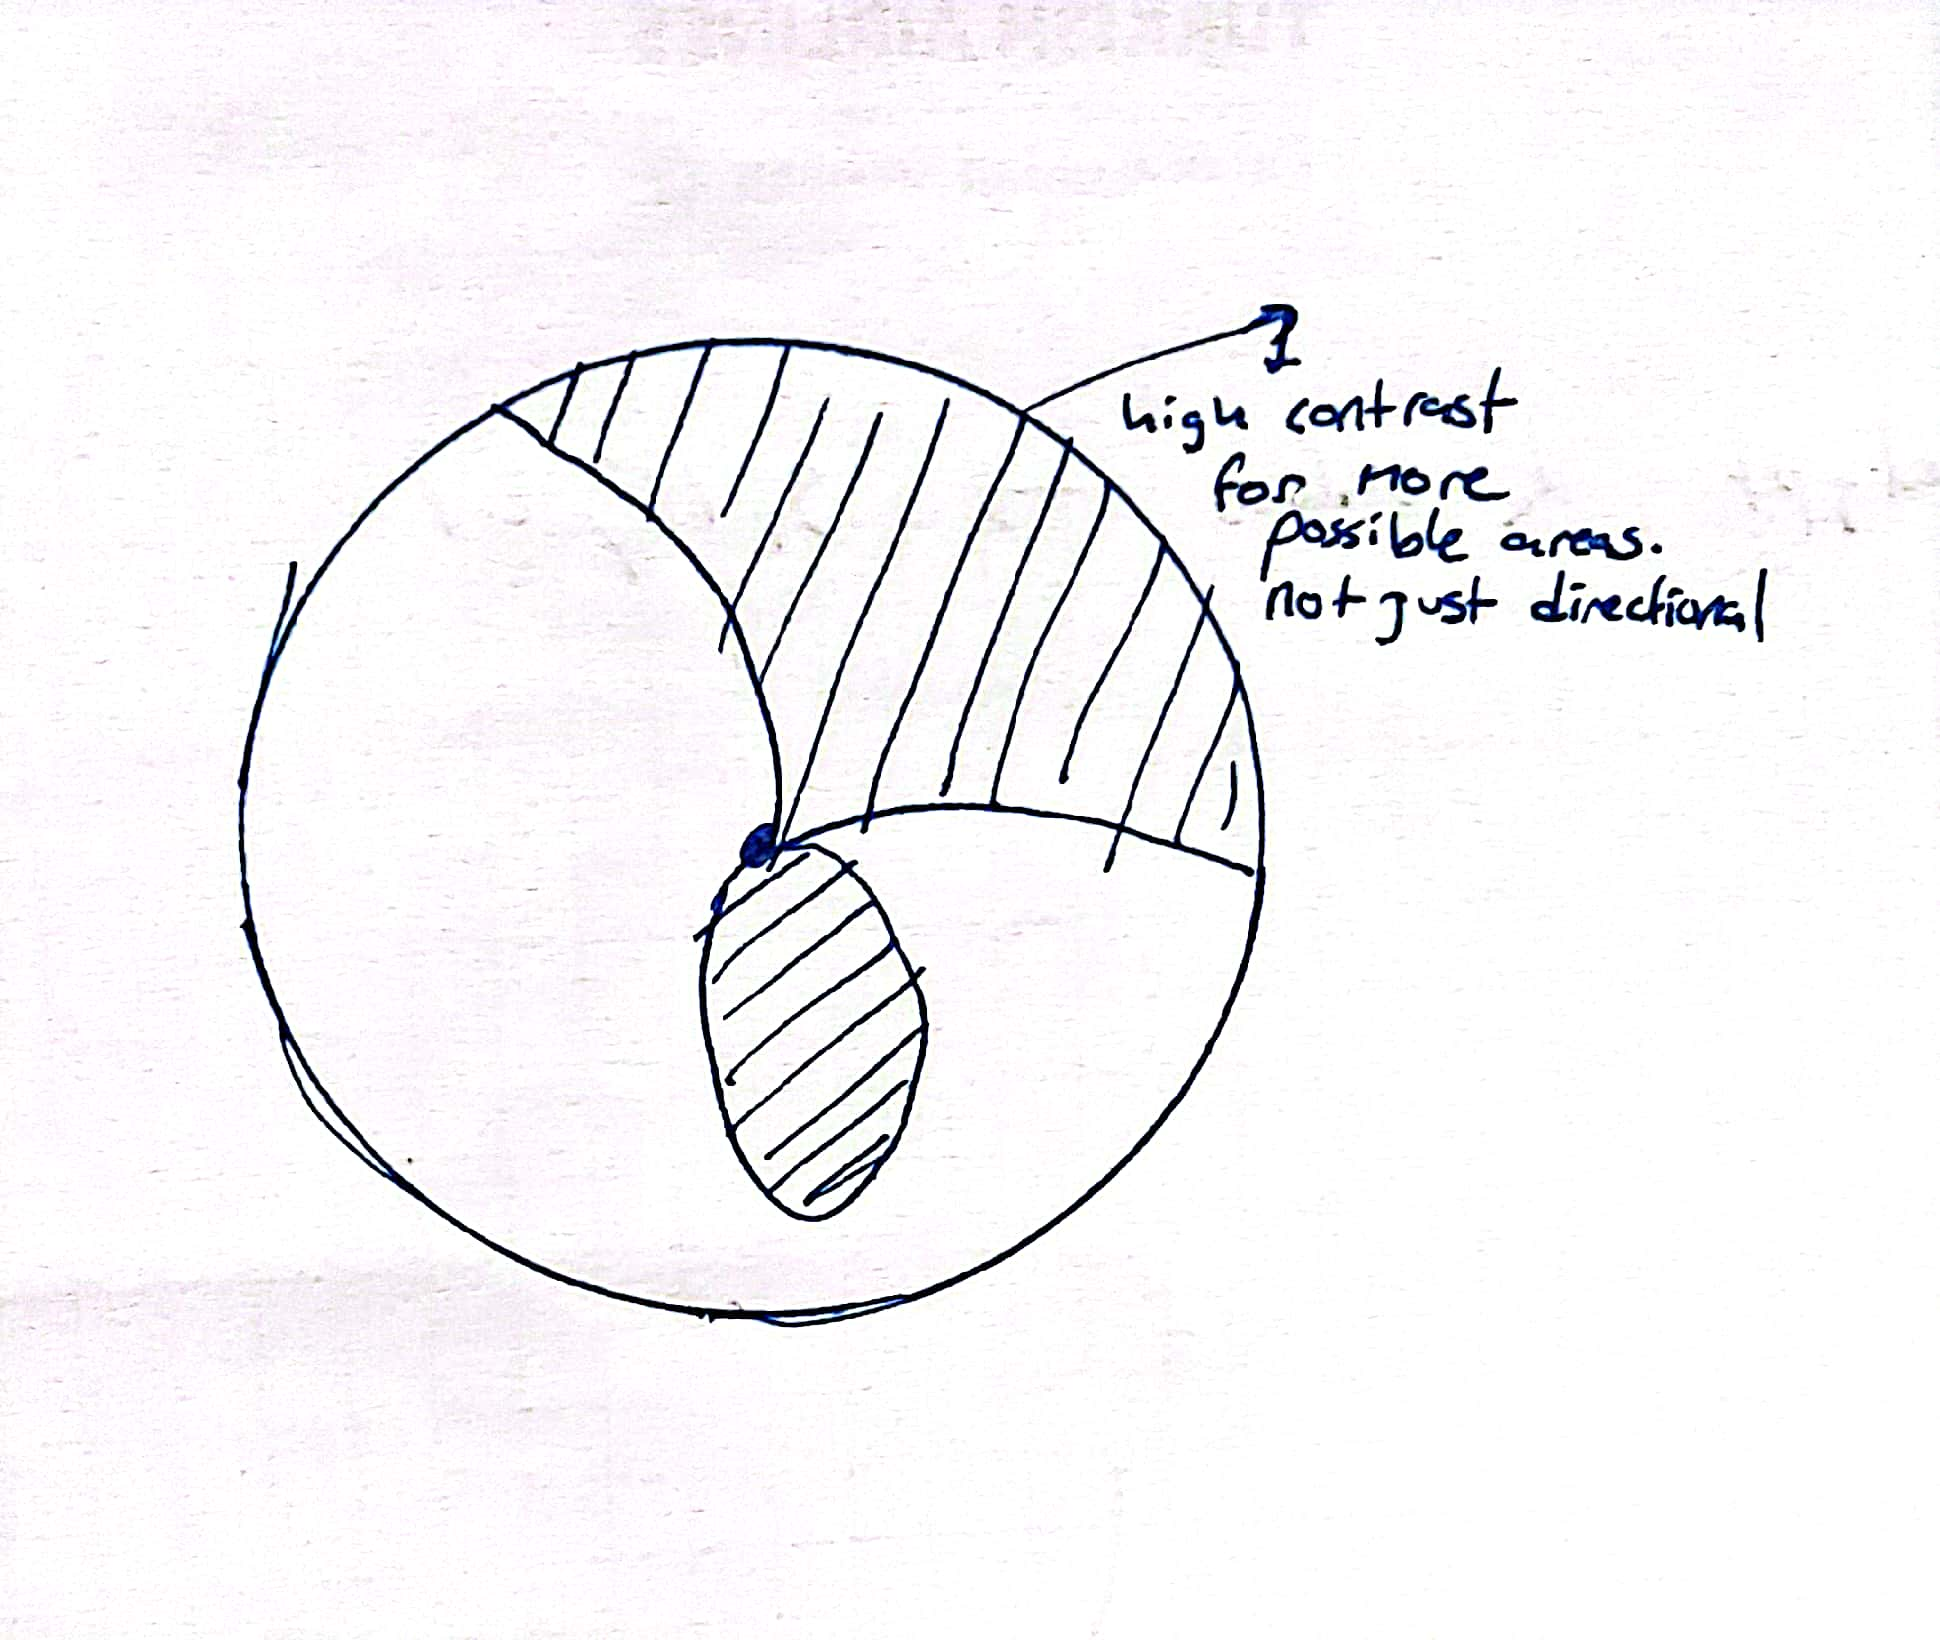
\includegraphics[width=0.95\columnwidth]{images/aeral-density.jpeg}
        \caption{Internal density-based concept. More likely subregions inside the uncertainty circle are shown with stronger contrast or denser shading, not only in a directional sense but also as localized high-probability areas.}
        \label{fig:aerial_density}
    \end{subfigure}

    \caption{Our proposed alternatives to the traditional uniform blue-dot uncertainty visualization.}
    \label{fig:our_visualization_ideas}
\end{figure}

At this stage, these ideas are still conceptual. However, they provide a useful basis for future prototyping and evaluation. In later stages of the project, we may refine these visual encodings and compare them in terms of interpretability, visual clarity, cognitive load, and usefulness in real map-based interaction scenarios.

\section{Implementation of our Visualization Methods}

\subsection{Input data format}

Our tool reads plain-text exports from the Android \textit{GNSS Logger} application. Each row of interest is a comma-separated line beginning with \texttt{Fix,} and follows the logger's column order (provider, latitude, longitude, altitude, speed, horizontal accuracy, bearing, Unix time in milliseconds, and further fields including vertical accuracy). For visualization we use only a subset: \textbf{latitude, longitude, altitude} for map placement and charts; \textbf{UnixTimeMillis} for temporal ordering; \textbf{AccuracyMeters} and \textbf{VerticalAccuracyMeters} for uncertainty views; and optionally speed and bearing where shown in the detail panel.

We use four prepared \texttt{Fix}-only extracts (each line is one fix). Sizes are summarized in Table~\ref{tab:fix_counts}.

\begin{table}[H]
    \centering
    \caption{GNSS Logger \texttt{Fix}-only datasets used in this work.}
    \label{tab:fix_counts}
    \small
    \setlength{\tabcolsep}{4pt}
    \begin{tabular}{@{} >{\raggedright\arraybackslash}p{0.62\columnwidth} r @{}}
        \toprule
        \textbf{Dataset} & \textbf{Lines} \\
        \midrule
        Tuzla Fix Only\newline
        \scriptsize\texttt{gnss\_log\_2026\_03\_23\_10\_52\_08\_FixOnly.txt} & 1209 \\
        \texttt{spor merkezi\_FixOnly.txt} & 595 \\
        \texttt{uc onu\_FixOnly.txt} & 601 \\
        \texttt{yuruyuske\_FixOnly.txt} & 610 \\
        \bottomrule
    \end{tabular}
\end{table}

A typical \texttt{Fix} row (fields we use are underlined conceptually in the description below) looks like:

\begin{quote}
\footnotesize
\raggedright
\begin{tabular}{@{}l@{}}
\texttt{Fix,GPS,40.8931388520,29.3753583357,170.0,}\\
\texttt{0.42999998,4.5,93.2,1774382541000,}\\
\texttt{0.66,136.0,210952725535317,5.0,0,,,\ldots}
\end{tabular}
\end{quote}

\noindent Here \texttt{40.893\ldots} and \texttt{29.375\ldots} are latitude and longitude in degrees; \texttt{170.0} is altitude in meters; \texttt{4.5} is horizontal accuracy (\texttt{AccuracyMeters}); \texttt{1774382541000} is \texttt{UnixTimeMillis}. Additional columns include vertical accuracy and other metadata used selectively in the UI.

\subsection{Web prototype}

We implemented an interactive prototype as a single-page web application (\texttt{gnss\_tuzla\_map\_interactive.html}) that loads Android GNSS Logger \texttt{Fix} lines and visualizes them on a Leaflet map with optional D3-based charts. A public build is hosted on GitHub Pages and can be opened directly in a browser:

\url{https://mufasa-349.github.io/Grad-Project-GPS-Data-Analysis/gnss_tuzla_map_interactive.html}

\begin{figure}[t]
    \centering
    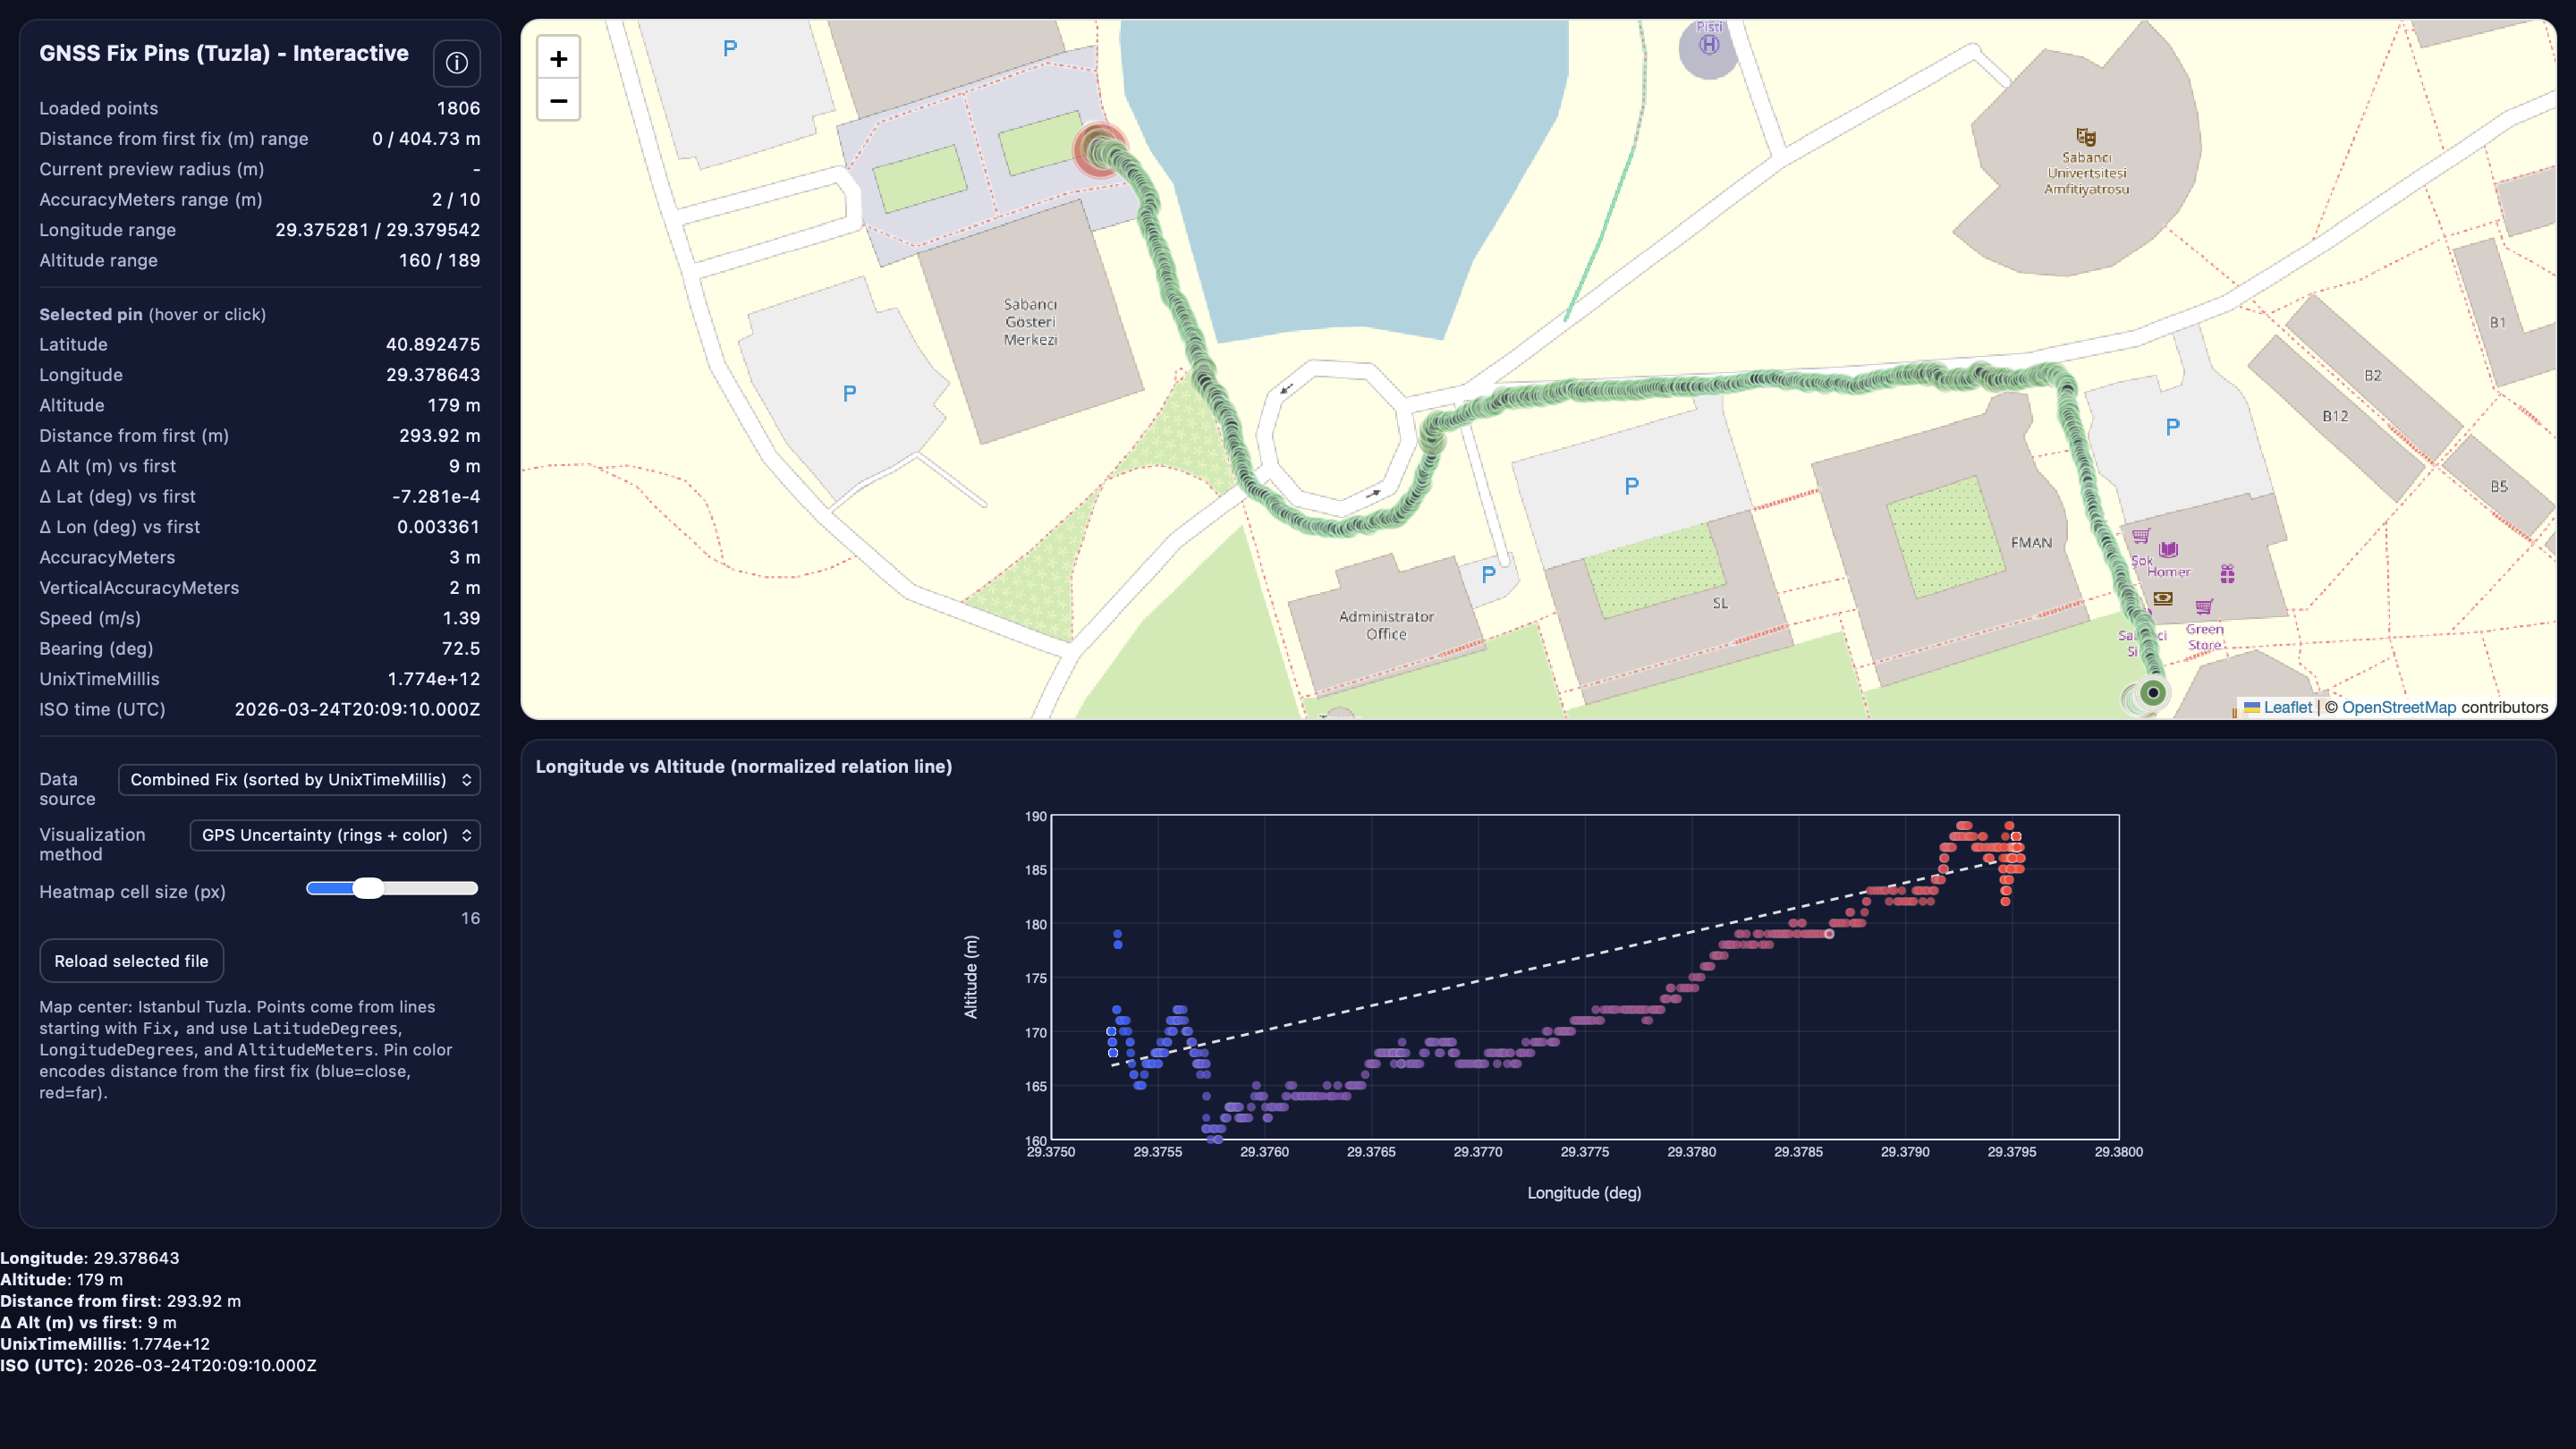
\includegraphics[width=\linewidth]{images/general-ui.png}
    \caption{Overview of the interactive GNSS visualization interface: control panel (left), map (top right), and longitude--altitude chart (bottom right).}
    \label{fig:general_ui}
\end{figure}

Figure~\ref{fig:general_ui} shows the main layout. The \textbf{left panel} summarizes the loaded dataset (point count, distance-from-first-fix range, accuracy ranges, altitude/longitude extents, and details for a selected point) and hosts the primary controls: \textbf{Data source} selects which prepared \texttt{Fix}-only or combined text file to load; \textbf{Visualization method} switches between the original point view, heatmap variants, and GPS uncertainty (accuracy rings); \textbf{Heatmap cell size} adjusts grid resolution where applicable; \textbf{Reload} refreshes the current file. The \textbf{(i)} button opens a short in-app ``How to use'' dialog. The \textbf{map} shows OpenStreetMap tiles with GNSS fixes overlaid according to the chosen mode (e.g., colored points, heatmaps, or uncertainty circles). The \textbf{lower chart} plots longitude versus altitude with a simple normalized regression line for quick inspection of the vertical profile. The tool is intended for exploratory analysis and comparison of uncertainty-centric views rather than for production navigation.

\begin{figure}[t]
    \centering
    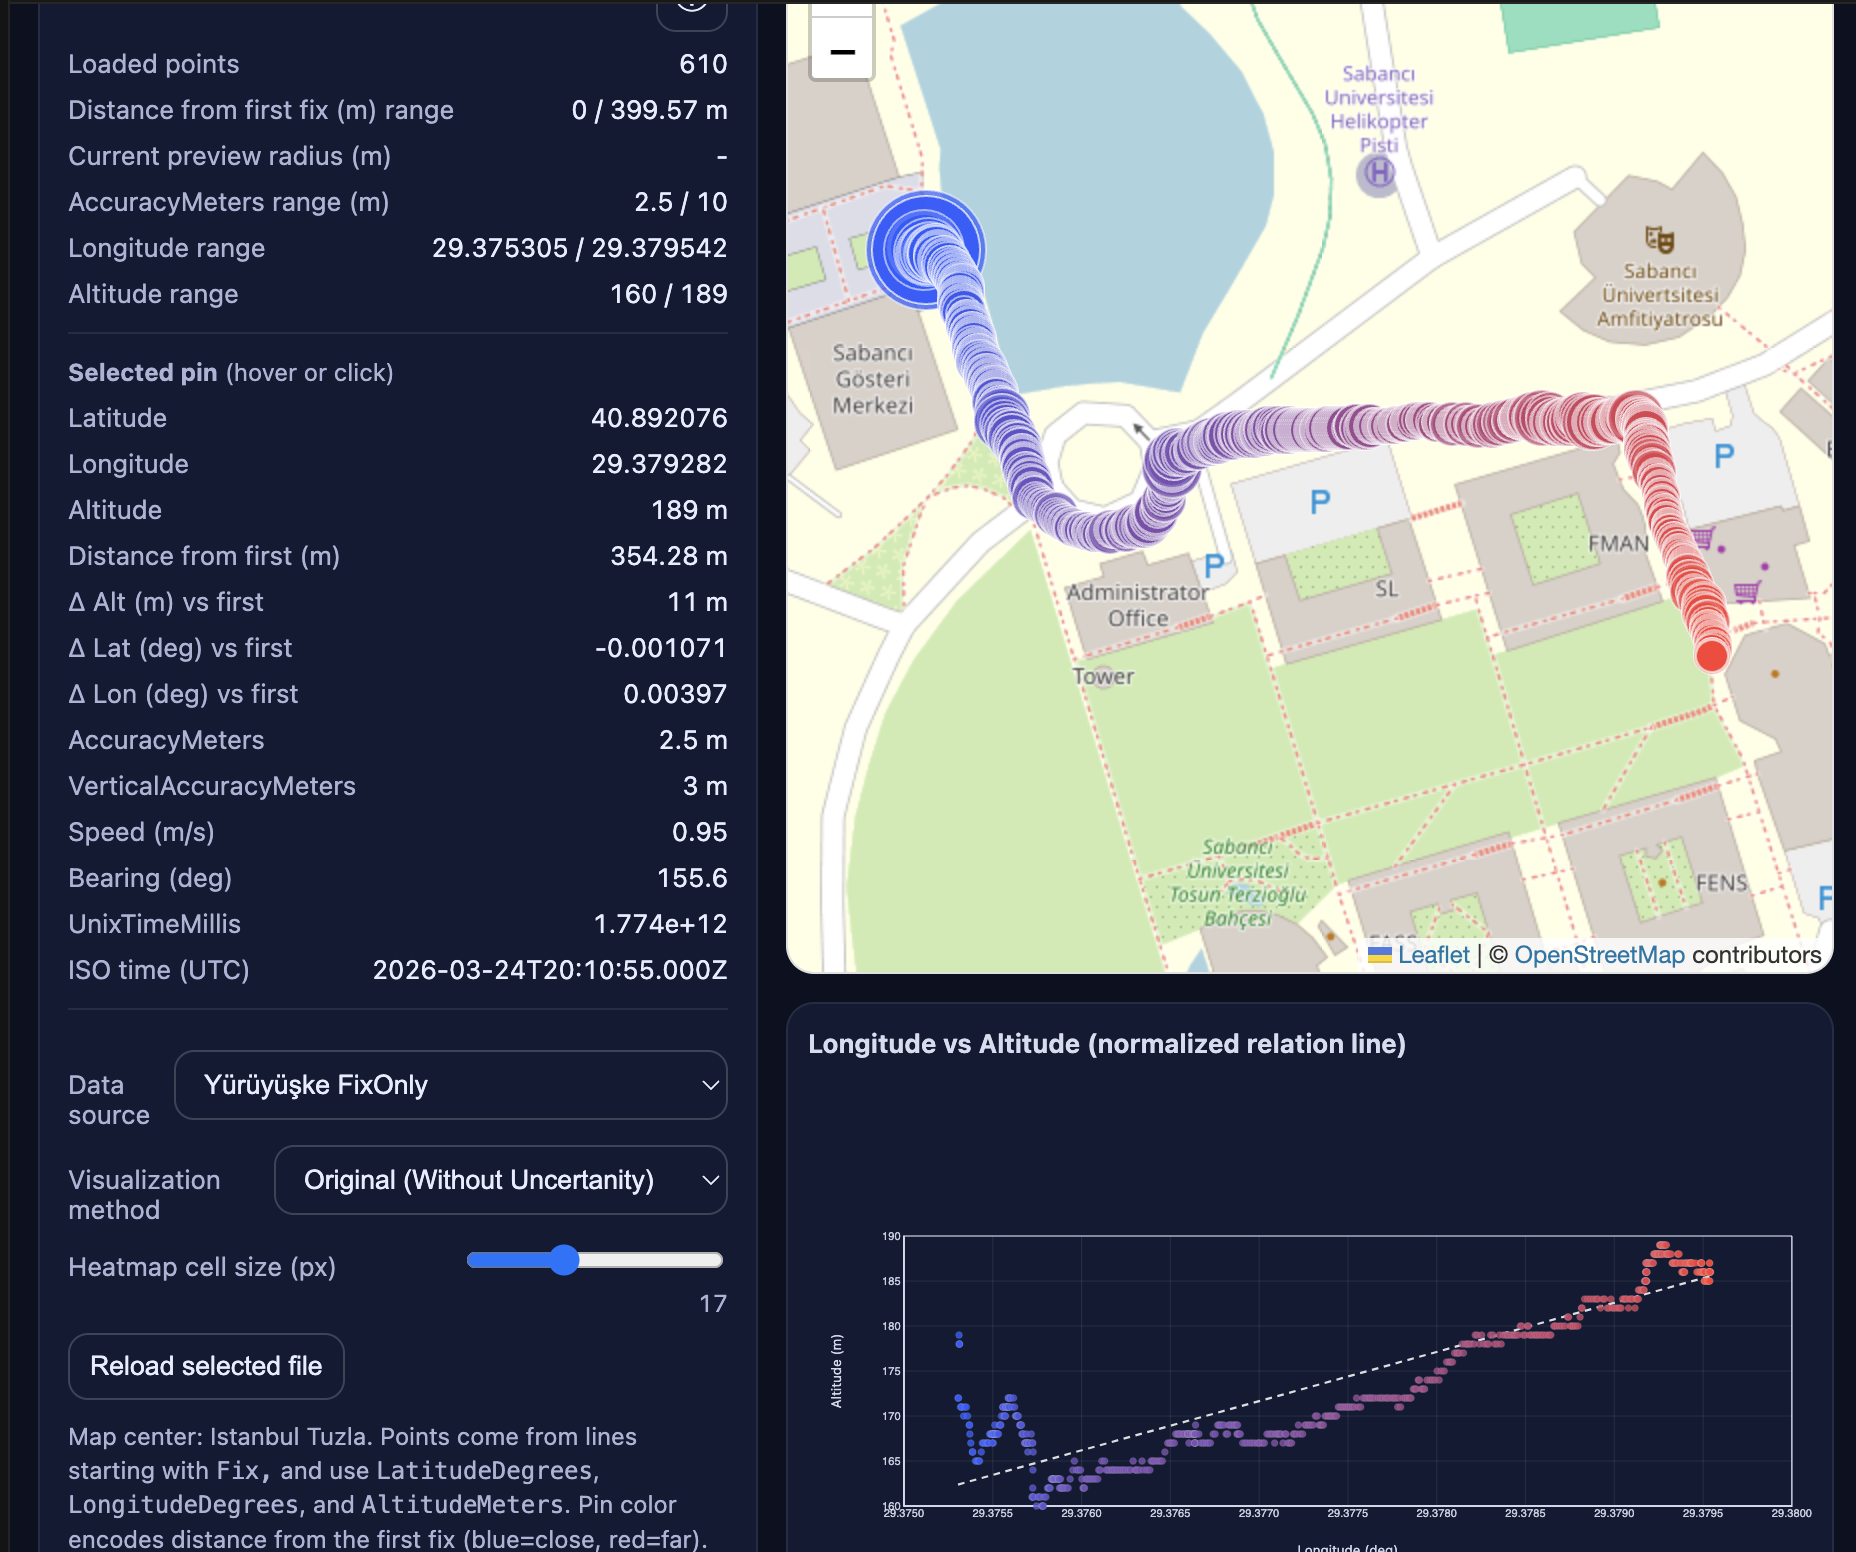
\includegraphics[width=\linewidth]{images/yuruyuske-original.png}
    \caption{Walking dataset \texttt{yuruyuske\_FixOnly}: approximately 35 minutes of GNSS fixes; the participant remained stationary for about 10 minutes at the start and end at the same location. The map uses the default \emph{point} mode: fixes are drawn at their reported latitude/longitude only---uncertainty is not visualized (no accuracy rings or other uncertainty overlays).}
    \label{fig:yuruyuske_original}
\end{figure}

Figure~\ref{fig:yuruyuske_original} illustrates this collection protocol: the dense clusters at both ends correspond to the standing-still segments, while the trace in between is the walk. The screenshot deliberately shows raw fix placement rather than an uncertainty-centric view, to establish a baseline before comparing other visualization modes.

For the \texttt{uc onu\_FixOnly} dataset we follow the same progression: first the default point view, then two heatmap encodings implemented in the prototype. The phone was held stationary for approximately 10 minutes; reported positions still wander, which motivates visualizing spread rather than a single crisp point.

\begin{figure}[H]
    \centering
    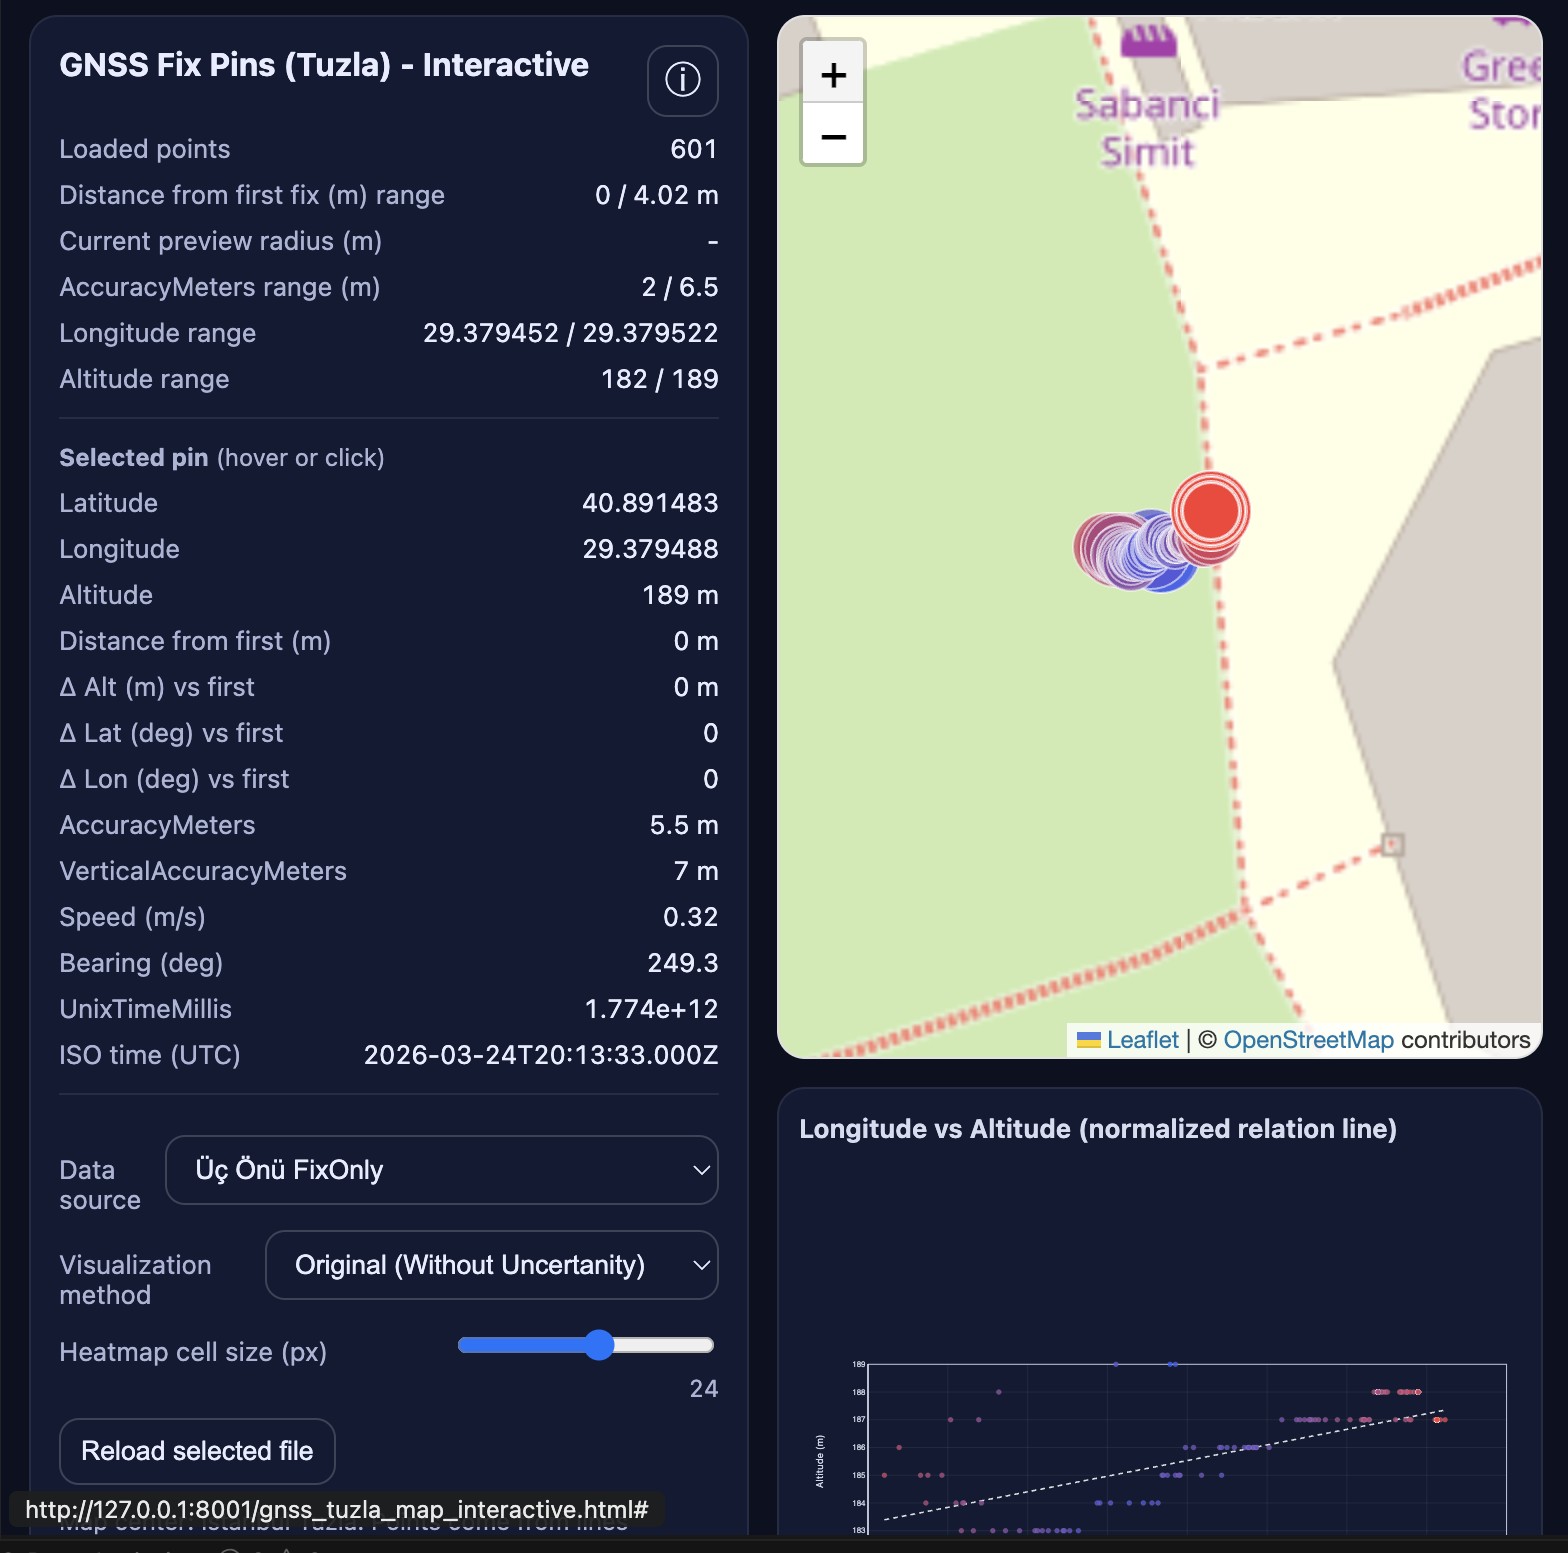
\includegraphics[width=\linewidth]{images/uc-onu-original.png}
    \caption{\texttt{uc onu\_FixOnly} (stationary hold, $\sim$10 minutes): default \emph{point} mode---each fix is plotted at its reported latitude/longitude with no uncertainty glyphs. Raw scatter under stillness is visible.}
    \label{fig:uc_onu_original}
\end{figure}

\begin{figure}[H]
    \centering
    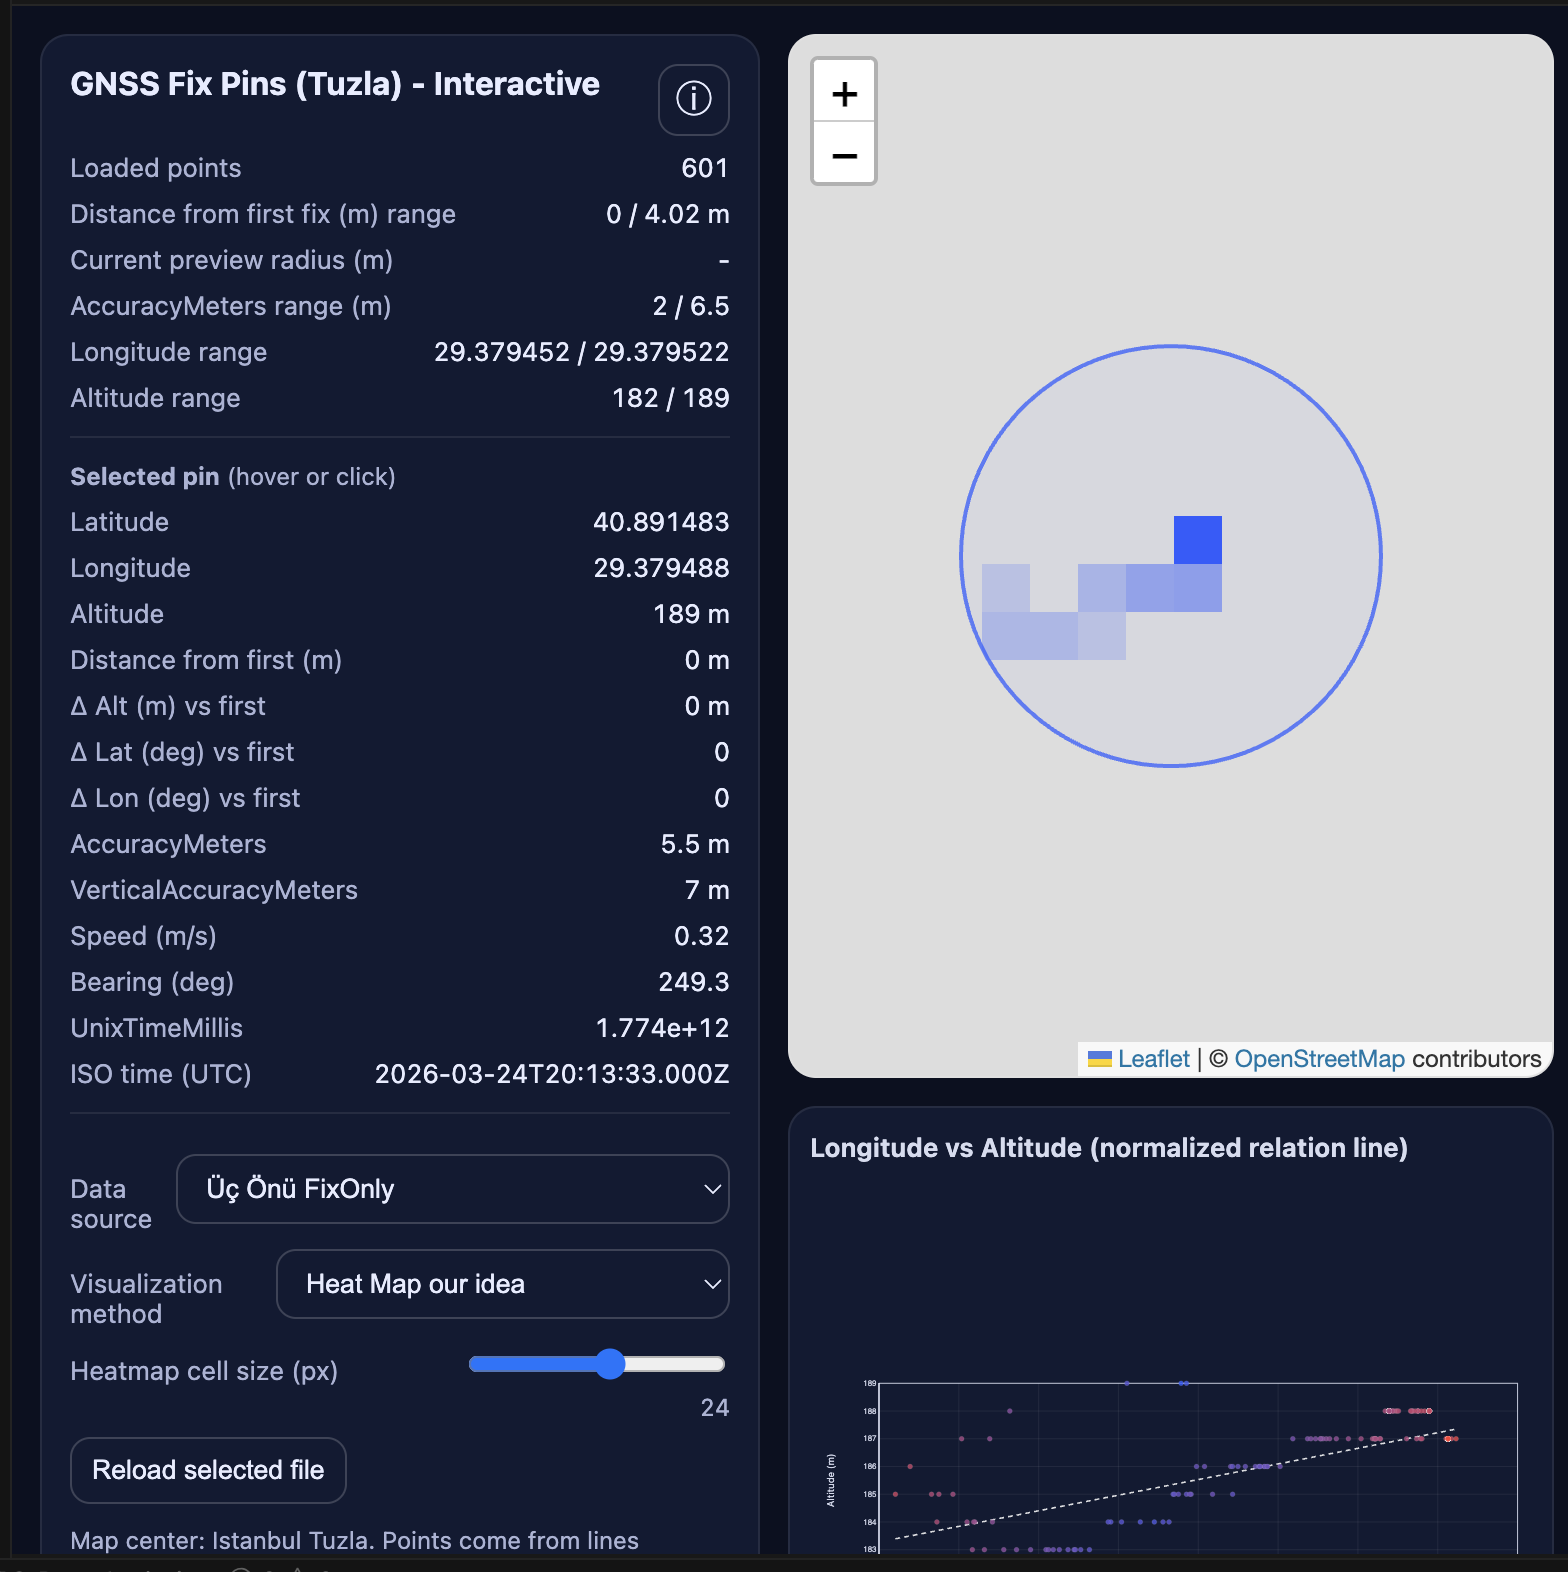
\includegraphics[width=\linewidth]{images/uc-onu-heatmap-our-idea.png}
    \caption{\emph{Heat Map our idea} on the same data. The tool bins screen-space fixes into a square grid (cell size set by the \emph{Heatmap cell size} control), counts fixes per cell, normalizes by the maximum count, and fills each nonempty cell with a fixed blue RGB while mapping normalized count to opacity (with a fractional power for contrast). A circle centered on the mean position encloses all fixes; rendering is clipped to that circle (stationary tracks use this single view).}
    \label{fig:uc_onu_heatmap_our_idea}
\end{figure}

\begin{figure}[H]
    \centering
    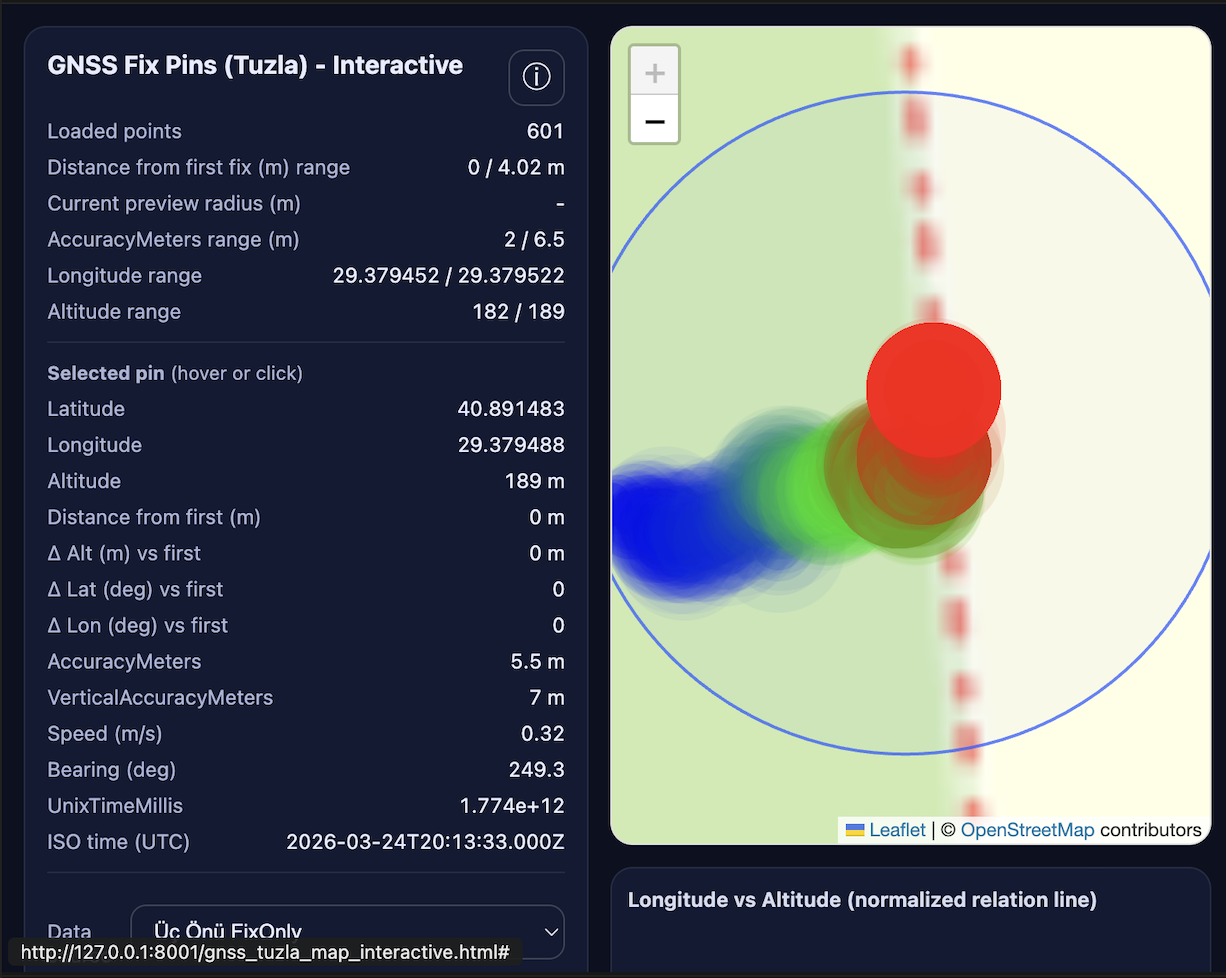
\includegraphics[width=\linewidth]{images/uc-onu-colored-heat-map.png}
    \caption{\emph{Heat Map (Blue--Green--Red)} on the same data. For each fix, the code computes a kernel density: a sum of Gaussian weights over all other fixes as a function of pairwise great-circle distance (meters), with scale tied to the spatial extent of the cloud. Densities are min--max normalized; hue runs blue $\rightarrow$ green $\rightarrow$ red with increasing density. Each fix is drawn as several semi-transparent concentric rings whose size and opacity depend on that normalized score, clipped to the same enclosing circle---a soft, marker-based heatmap rather than a screen grid.}
    \label{fig:uc_onu_heatmap_bgr}
\end{figure}

Figure~\ref{fig:uc_onu_original}--\ref{fig:uc_onu_heatmap_bgr} summarize the comparison: Figure~\ref{fig:uc_onu_original} shows unstructured scatter; Figure~\ref{fig:uc_onu_heatmap_our_idea} emphasizes \emph{where} fixes pile up on a coarse grid; Figure~\ref{fig:uc_onu_heatmap_bgr} emphasizes local crowding via kernel density and a sequential blue--green--red hue scale. Neither heatmap substitutes for explicit accuracy rings (that is a separate \emph{GPS Uncertainty} mode in the tool), but both make positional ambiguity visually salient from the fix cloud alone.

Finally, we return to the walking dataset \texttt{yuruyuske\_FixOnly} (cf.\ Figure~\ref{fig:yuruyuske_original}) for two additional views placed here for narrative closure before the conclusion.

\begin{figure}[H]
    \centering
    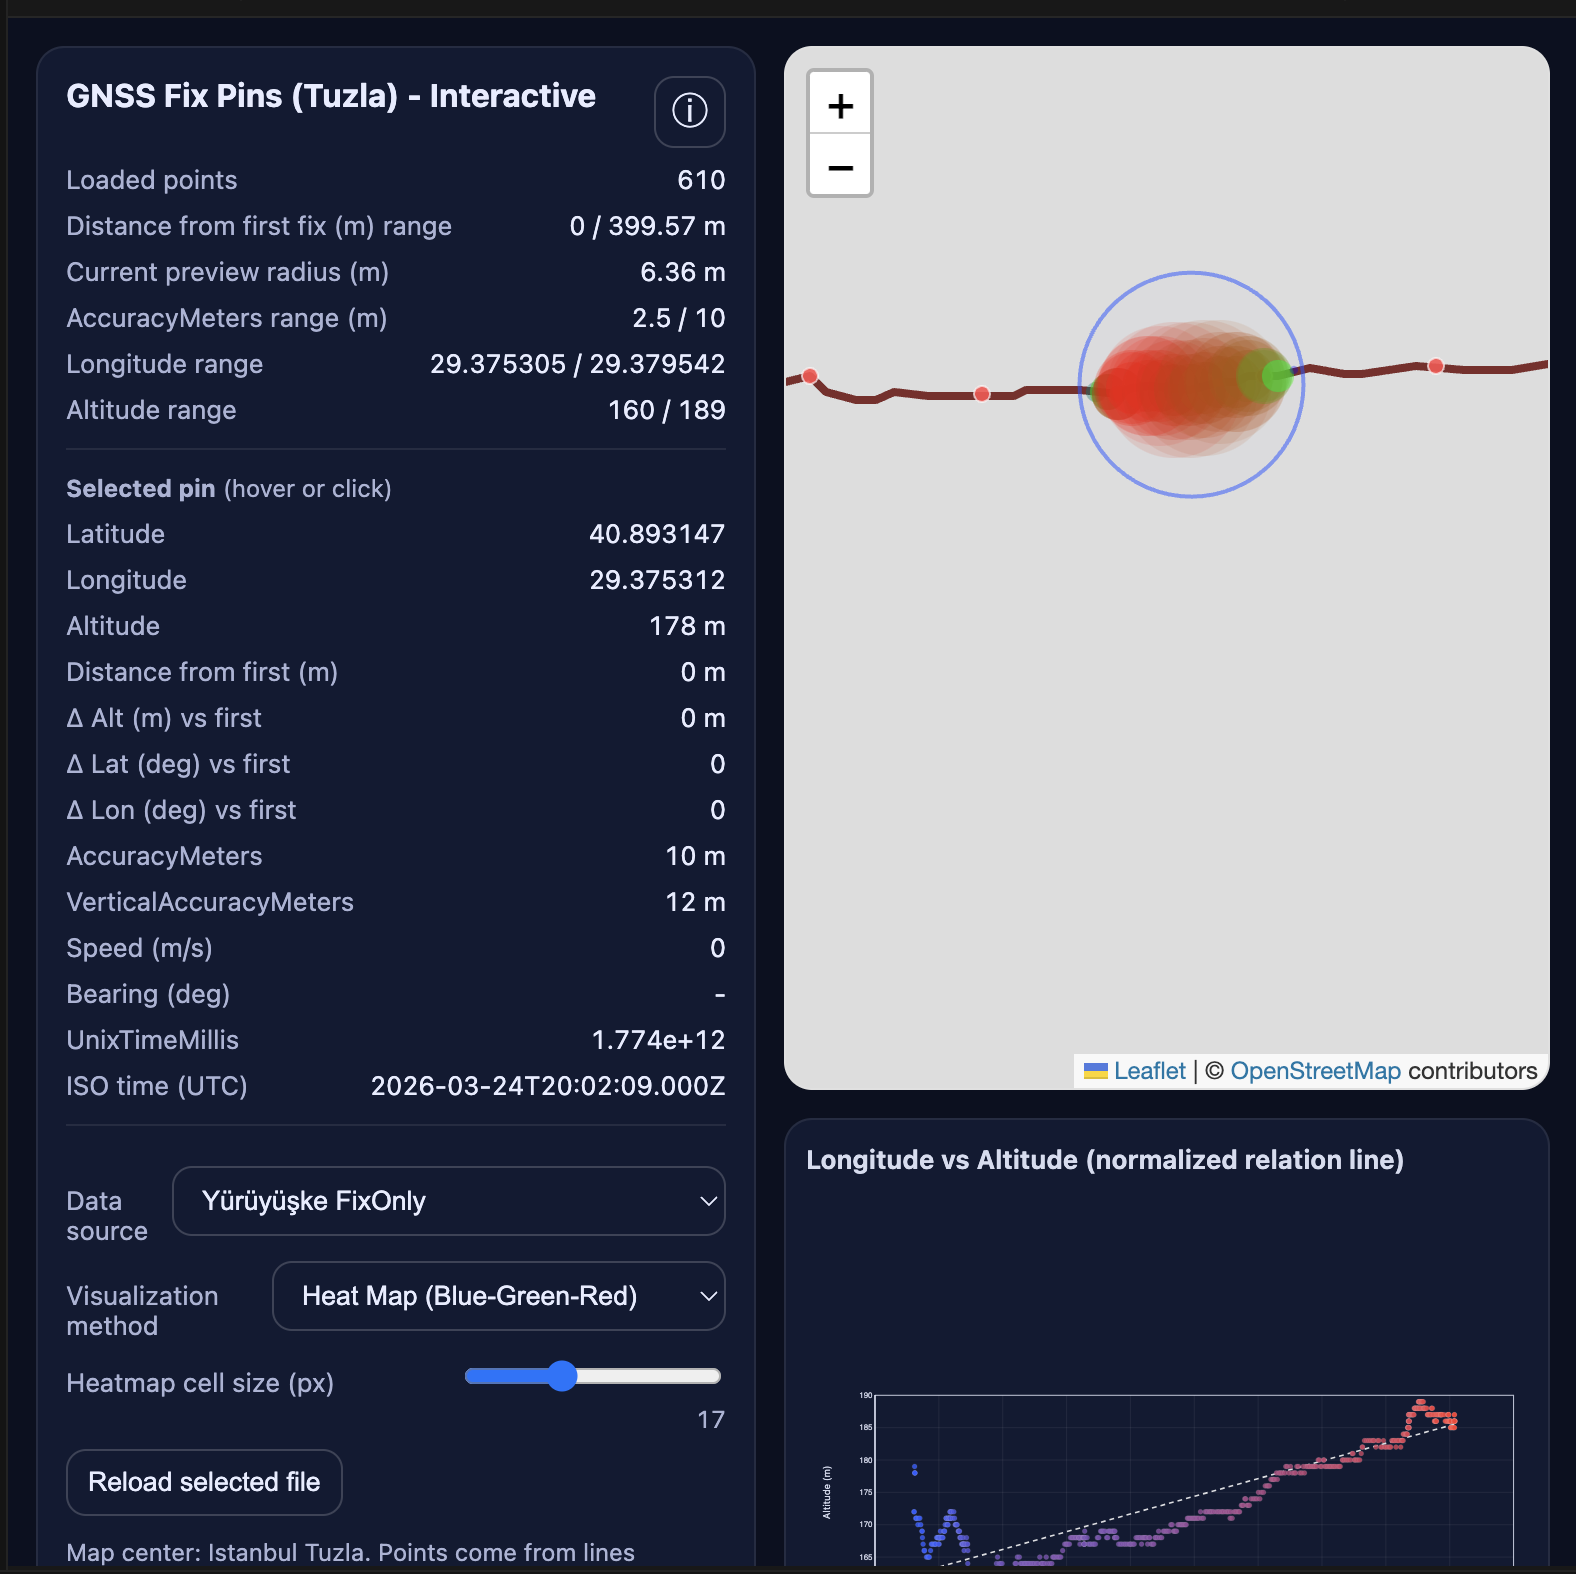
\includegraphics[width=\linewidth]{images/yuruyuske-heatmap-colored.png}
    \caption{The same walking dataset \texttt{yuruyuske\_FixOnly} using \emph{Heat Map (Blue--Green--Red)}: the same kernel-density, sequential hue encoding as in Figure~\ref{fig:uc_onu_heatmap_bgr}, applied here along the full trajectory so that segments with tighter fix crowding read hotter (green/red) and sparser segments cooler (blue).}
    \label{fig:yuruyuske_heatmap_bgr}
\end{figure}

\begin{figure}[H]
    \centering
    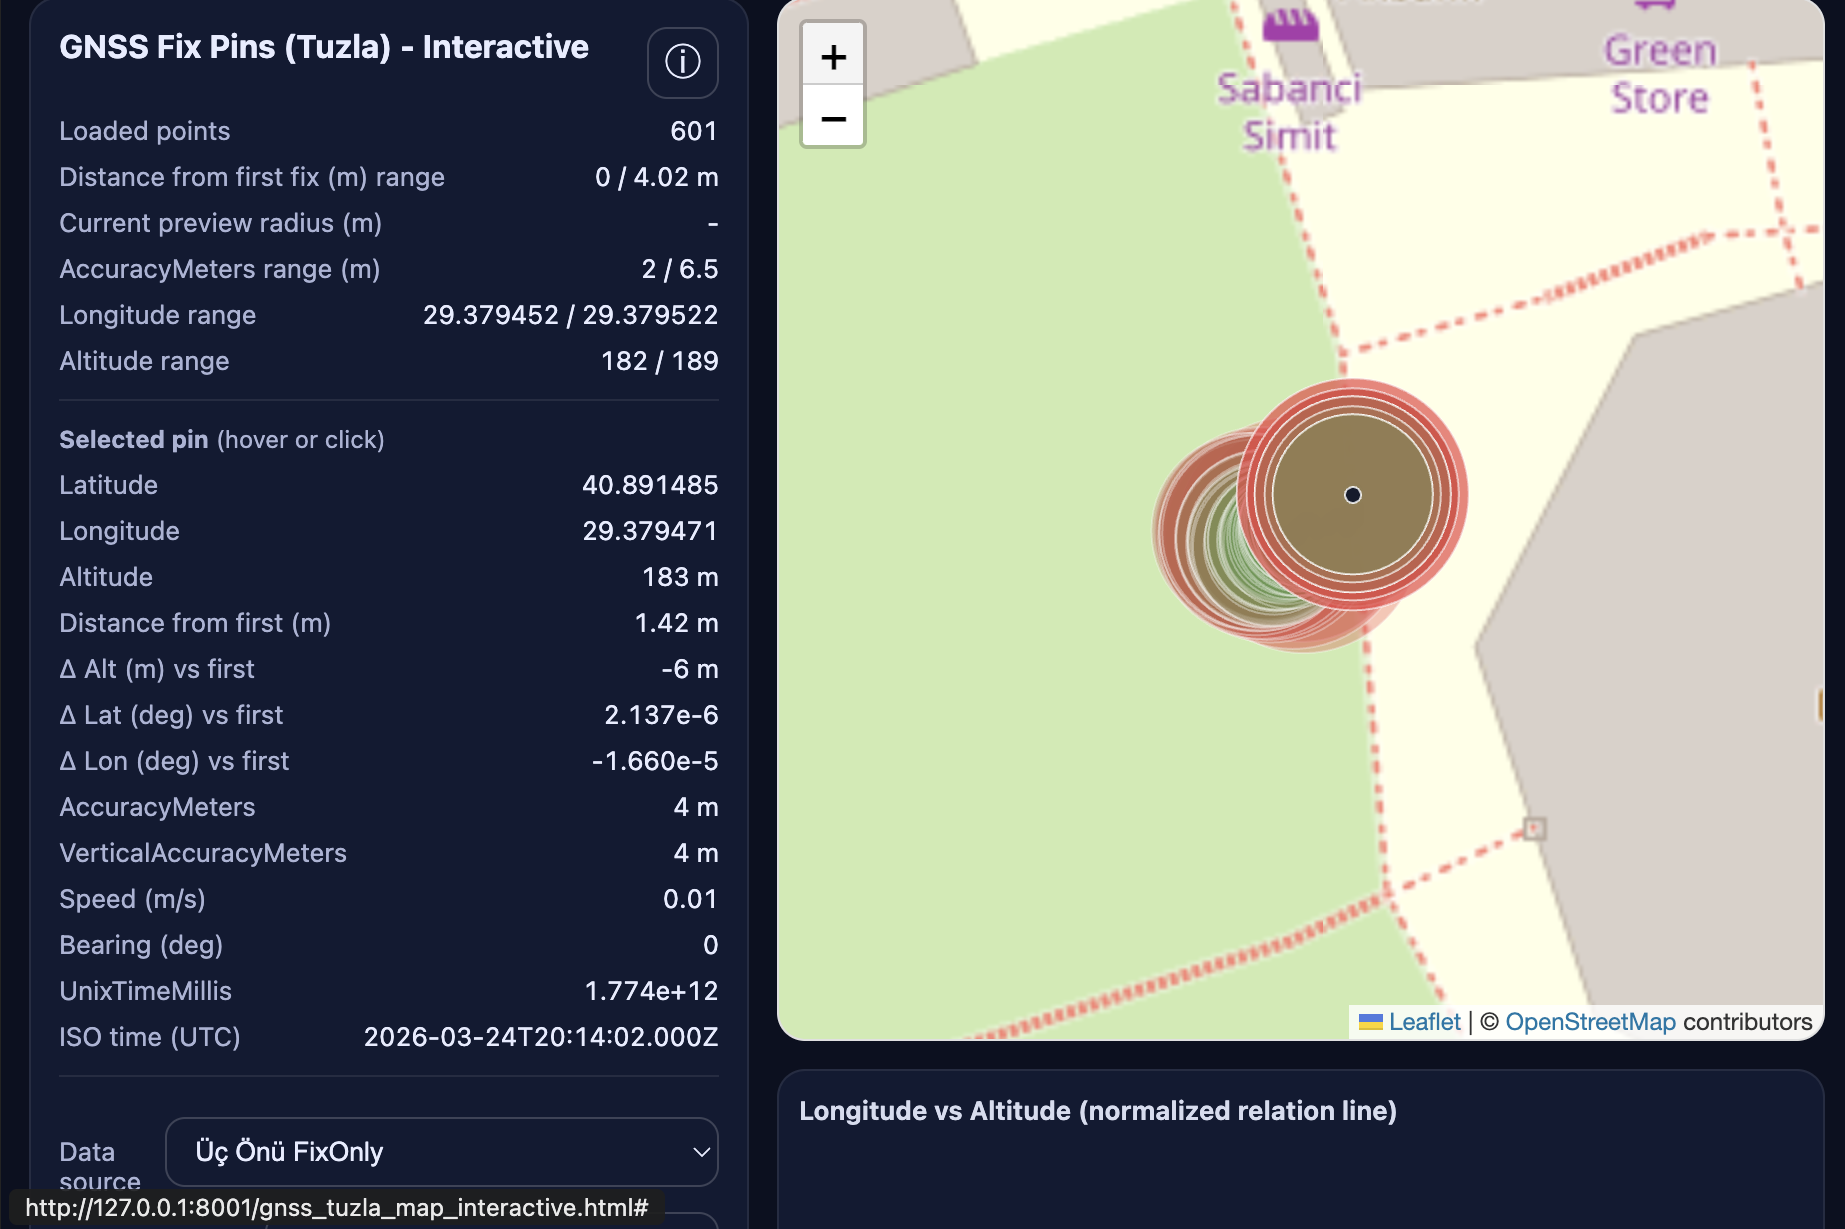
\includegraphics[width=\linewidth]{images/yuruyuske-ai-idea.png}
    \caption{Exploratory visualization for \texttt{yuruyuske\_FixOnly} produced from an \emph{AI-suggested} design direction (concept sketch rather than a finalized project commitment). This encoding is included as a placeholder example only and \textbf{may be replaced} by a stronger, fully original manual design as the work matures.}
    \label{fig:yuruyuske_ai_idea}
\end{figure}

Figure~\ref{fig:yuruyuske_heatmap_bgr} contrasts the raw point baseline in Figure~\ref{fig:yuruyuske_original} with density-aware color along the walk. Figure~\ref{fig:yuruyuske_ai_idea} documents an optional AI-assisted idea for the same route; we do not treat it as fixed scope---it can be swapped for a better original visualization without changing the core research goals.

\section{Conclusion}

This mock proposal establishes the initial direction of a study on visualizing uncertainty in GPS and location-based data. The project focuses on making uncertainty visible rather than hiding it, so that users can interpret positional information more realistically. The reviewed literature shows that visual encoding choices strongly affect how users understand uncertain position estimates, especially in navigation and self-location tasks. The next step is to expand the literature coverage where needed and then derive concrete visualization proposals based on the most relevant design patterns.

\clearpage
\bibliographystyle{IEEEtran}
\bibliography{references}

\end{document}